\documentclass[preprint,12pt]{elsarticle}
\usepackage[T1]{fontenc}
\usepackage[utf8]{inputenc}
\usepackage{graphicx}
\usepackage{multirow}
\usepackage{amsmath,amssymb,amsfonts}
\usepackage{amsthm}
\usepackage{mathrsfs}
\usepackage{xcolor}
\usepackage{textcomp}
\usepackage{booktabs}
\usepackage{array}
\usepackage{caption}
\usepackage{subcaption}
\usepackage{algorithm}
\usepackage{algpseudocode}
\usepackage{mathtools}
\usepackage{hyperref}
\usepackage{tikz}
\usetikzlibrary{arrows.meta,positioning,shapes.geometric}
\graphicspath{{./}}
\theoremstyle{plain}
\newtheorem{theorem}{Theorem}
\newtheorem{proposition}{Proposition}
\setlength{\emergencystretch}{3em}
\usepackage{microtype}
\journal{Signal Processing: Image Communication}
\biboptions{numbers,sort&compress}
\begin{document}
\begin{frontmatter}
\title{Bounded Intra-Cover Hash Assignment for Coverless Image Steganography}
\author[aff1]{Habibatou Mindja}
\ead{habibatoumindja@yahoo.fr}
\author[aff2]{Ibrahima Tour\'e}
\ead{astourep@gmail.com}
\author[aff1,aff4]{St\'ephane Ga\"el R. Ekodeck}
\ead{stephane-gael.ekodeck@facsciences-uy1.cm}
\author[aff1,aff4]{Serge Alain Ebele}
\ead{serge-alain.ebele@facsciences-uy1.cm}
\author[aff1,aff4]{Leonel Moyou Metcheka}
\ead{leonelmoyou@gmail.com}
\author[aff1]{Daniel Tieudjo}
\ead{tieudjo@yahoo.fr}
\author[aff3,aff4]{Ren\'e Ndoundam\corref{cor1}}
\ead{ndoundam@gmail.com}
\cortext[cor1]{Corresponding author}

\address[aff1]{University of Yaound\'e I, LIRIMA, Team GRIMCAPE, P.O. Box 812, Yaound\'e, Cameroon}

\address[aff2]{Institut Sup\'erieur des Technologies de Mamou, B.P. 063, Mamou, Republic of Guinea}

\address[aff3]{University of Bertoua, P.O. Box 416, Bertoua, Cameroon}

\address[aff4]{IRD, UMI UMMISCO, IRD France Nord, F-93143 Bondy, France}
\begin{abstract}
FHAM is an intra-cover assignment layer for coverless mapping. Sender and receiver share an unchanged image as a hash-location reference; an external AES-256-GCM-protected location--residual record supports reconstruction. Given a message and fixed-cover codebook, FHAM assigns symbols injectively with residuals bounded by $B$ and minimizes their total absolute value through rectangular linear assignment. Hall's condition characterizes feasibility. With raw message bytes and $B=2$, assignment feasibility reaches 100\% through 200 symbols on eight controlled images and 74.4\% at length 200 on a 219-image stress corpus. At length 200, raw-message feasibility is 100\% for uniform-byte and printable-ASCII messages, 12.5\% for templated text, and 0\% for repeated-byte messages, showing that effective capacity depends on symbol multiplicities. Without source preprocessing, the compact protected record in a matched $B=2$, 200-symbol cohort averages 549.88 bytes, compared with 230.10 bytes for direct protection of the message; the fixed-capacity shaped record is 852 bytes.
An ablation of lossless pre-assignment compression and codebook parameters identifies a spectral $12\times12$-block profile: on 200 LFW covers, zlib preprocessing raises $B=2$ feasibility from 0\% to 97.8\% for repeated-byte messages and from 80.5\% to 92.2\% for templated text (600 image--message cases per family). A separate 11-image scene holdout reaches 100\% for repeated-byte messages and 97.0\% for templated text, with 33 cases per family. A packed-record prototype reduces protected metadata size, while the measured FHAM records remain larger than directly protected, equivalently compressed messages.
In a separate transport evaluation against captured NonVPN TLS flows, a detector combining directional TLS record counts, byte totals, and the first 16 record lengths reached mean AUC 0.976, while size-matched HTTP controls yielded AUC 0.50. An empirical padding and fragmentation profile reduced the combined byte-total/record-count detector AUC from 0.929 to 0.781; the detector using counts, totals, and the first 16 record lengths reached AUC 0.955.
\end{abstract}
\begin{keyword}
coverless image steganography \sep intra-cover mapping \sep bounded assignment \sep bipartite matching \sep Hall's theorem \sep combinatorial optimization
\end{keyword}
\end{frontmatter}
\section{Introduction}
Steganography conceals the existence of secret communication within an innocuous carrier \cite{johnson1998exploring}. Conventional image steganography modifies pixel or transform coefficients, for example through least-significant-bit substitution \cite{chan2004hiding}. Even small modifications can create statistical evidence exploitable by modern steganalysis \cite{fridrich2012rich,xu2016structural}.

Coverless image steganography (CIS) avoids this modification channel by representing data through intrinsic image features or generated content \cite{zhou2015coverless,qin2020gan,tan2024review}. Mapping-based CIS commonly indexes images or image regions by robust hash sequences \cite{zheng2018coverless}. Its practical capacity depends on nominal hash length together with the availability and multiplicity of values in the selected cover.

The architecture evaluated here uses a shared preprocessed image as a reference dictionary of hash-indexed locations. Its pixels remain unchanged across message assignments; the external AES-GCM-protected auxiliary record carries the selected locations and signed residuals required for reconstruction. We use the term coverless image steganography to identify this mapping paradigm, and focus on the assignment layer within it. Image-only concealment and end-to-end transport are properties of the surrounding protocol.

For secure multimedia communication, fixed-cover CIS creates a distinct assignment problem: given a cover and a message, determine whether each message value can be assigned to a distinct intrinsic location under a specified residual bound, and find a minimum-cost assignment when one exists. Feasibility depends on demand multiplicity and neighboring hash-location capacity: exact matching can leave locations unused when a message demands a value more often than that exact hash occurs. FHAM formalizes this fixed-cover assignment and measures its metadata cost alongside direct encryption. Its value is a formally characterized assignment component for architectures that require a shared, unchanged cover and location-level representation; transport concealment, cover selection, and synchronization remain surrounding protocol functions.

This paper isolates a precise intra-cover assignment problem. In an exact-match design, a symbol requires an unused location with the same 8-bit hash, so available locations may remain unusable for a particular message. The central question is whether those locations can be assigned under an explicit residual bound while retaining deterministic reconstruction. The descriptor supplies the location/hash codebook; FHAM assigns message symbols to distinct locations and records residuals; encryption and authentication protect that record; and the surrounding transmission protocol handles key establishment, transport, concealment, and synchronization. Our experiments characterize assignment behavior and selected metadata properties within this layered architecture.

The assignment is coupled across message positions: choosing a location for one
symbol removes it from the choices available to every other symbol. The total
number of image locations therefore does not determine feasibility; a subset
of repeated or nearby symbol values can compete for too few neighboring hash
locations, precisely the obstruction captured by Hall's condition. A
symbol-by-symbol nearest match can also consume a location needed by a more
constrained symbol. The bounded model gives an exact feasibility criterion and
a globally minimum-residual solution for this fixed-cover setting, while the
message-family experiments measure how symbol multiplicities determine its
effective capacity. These properties define the assignment primitive studied
here; the measured record-size results characterize its communication cost.
The direct AES-GCM baseline is smaller in the tested byte-count comparison;
FHAM therefore makes no claim of payload-efficiency or confidentiality gains
over direct encryption. Its scientific contribution is the exact
cover-conditioned assignment capability: the causal ablation shows that
bounded global assignment recovers feasible mappings that exact matching
cannot construct under the same codebooks.

\subsection{Contributions}
We answer this question with \textit{Flexible Hash-to-ASCII Mapping} (FHAM), an assignment-layer method that takes a message and a descriptor-generated fixed-cover codebook as input. The image is unchanged; the message-reconstruction record is external and protected separately. The feature descriptor supplies the location/hash codebook, FHAM computes the bounded injective assignment, AES-256-GCM protects the external record, and the surrounding protocol handles cover delivery, key establishment, traffic concealment, and synchronization. The contributions are:
\begin{enumerate}
    \item \textbf{Bounded feasibility model:} We model intra-cover mapping as an injective assignment with $|\delta_j|\leq B$ and characterize feasibility through Hall's condition. The unbounded capacity result follows as a special case.

    \item \textbf{Global displacement optimization:} We formulate minimum-displacement mapping as a rectangular linear assignment problem with cost $c_{jp}=|\alpha_j-h(p)|$. The implemented rectangular assignment solver returns the global $L_1$ optimum.

    \item \textbf{Codebook geometry:} We use the covering radius and the complete gap structure, rather than codebook density alone, to characterize unconstrained nearest-neighbor displacement.

    \item \textbf{Reproducible comparative validation:} We compare exact matching, bounded and global assignment, Abdulsattar's overlapping Arr.4 mapping, and the WYSAWIS block/category mapping on eight standard images and a 219-image stress corpus. The evaluation includes a minimum-bottleneck baseline, a randomized feasible baseline, a dense-versus-aggregated-flow equivalence check, a causal ablation crossing four codebooks (three FHAM descriptors and Abdulsattar's) with the same assignment strategies, a three-descriptor comparison followed by a validation-gated selection frozen on a disjoint BOSSBase sample, a five-point stability-aware $\lambda$ sweep evaluated under disjoint development/validation transformations, a block-size, descriptor, displacement-bound, and message-preprocessing ablation on 200 LFW covers with a separate scene holdout, the complete four-family eight-length message manifest, a message-length leakage measurement, a 36-condition extended transformation matrix, a 180-image external check, and a stratified robustness check at larger scale across BOSSBase, BOWS2, and COCO~2017. Assignment feasibility and post-transformation recovery are reported as separate metrics.

    \item \textbf{Audited assignment representation:} We serialize and protect the location--residual records to quantify the metadata required by the assignment layer and establish a reproducible implementation reference.
\end{enumerate}

\subsection{Organization}
Section \ref{sec:related} identifies the gap in existing CIS mappings. Section \ref{sec:formal_model} develops the assignment model and guarantees. Section \ref{sec:methodology} translates the model into the FHAM assignment procedure and record representation. Section \ref{sec:experiments} evaluates the resulting assignment method, and Section \ref{sec:conclusion} concludes.

\section{Related Work}
\label{sec:related}

\subsection{Mapping- and Generation-Based CIS}
Coverless image steganography (CIS) is commonly organized into mapping-based and generation-based families. Recent surveys identify capacity, robustness, security, and practical deployment as persistent evaluation dimensions and document the expansion of both low-level-feature and semantic/deep-learning approaches \cite{tan2024review,xiang2025survey,zhang2026diffusion}. Mapping-based CIS associates secret segments with pre-existing images or image features, while generation-based CIS synthesizes content conditioned on the secret. The original mapping framework selected natural images whose robust hashes match message segments \cite{zhou2015coverless}; later work strengthened image retrieval and robustness through structured hashes and local descriptors \cite{zheng2018coverless,li2024surf}. More recent systems diversify hash sequences against passive and active analysis \cite{guo2024diverse}, combine selection and generation modules \cite{ren2024joint}, or target robustness near dataset-level capacity through stability-aware quantization and clustering \cite{guo2026capacity}.

Generation-based methods follow a different carrier model. GAN-based CIS synthesizes images from secret-conditioned representations \cite{qin2020gan}, while recent diffusion-oriented reviews emphasize image quality, robustness, capacity, and security as separate design axes \cite{zhang2026diffusion}. A 2026 CVPR Findings approach uses multimodal large language models to map secret messages to semantic features compatible with black-box image generators, explicitly targeting universality and reduced local resource dependence \cite{li2026mllm}. These advances are important for end-to-end CIS, but they do not address the fixed-cover, location-level assignment problem studied here.

Related feature-learning studies explore complex-scene recognition. Learned
representations for human parsing and mask-guided visible--infrared feature
fusion for aerial vehicle detection illustrate task-specific approaches to
robust features \cite{liu2024humanparsing,wang2024maskmamba}. These approaches
may motivate future descriptor design; transfer to FHAM block-hash
repeatability under rotation or cropping remains an empirical question.

Watermarking and forensic methods address related but distinct signal models.
Screen-shooting watermarking methods recover an embedded signal after capture
or display transformations \cite{fu2025waverecovery,li2024screenshooting};
FAMM detects compressed deepfake video from facial-motion features
\cite{liao2023famm}, while orthogonal-moment watermarking supports proactive
deepfake detection \cite{wang2026orthowatermark}. These works provide context
for robust recovery and forensic detection; FHAM's evaluated architecture
pairs an unchanged cover with an external encrypted record. Recent chaotic
image/video encryption work studies multimedia encryption and keystream
construction \cite{gao2025memristive,gao2025story,gao2025chaosreview}.
This study evaluates AES-GCM for the auxiliary byte record; alternative
multimedia encryption constructions call for record-specific comparison of
authentication, nonce handling, and key management.

\subsection{Database Retrieval and Multi-Cover Allocation}
Database-retrieval-oriented methods select one or more carriers from a shared
image collection by matching message-derived features to indexed image
features; their central resource is the searchable cover corpus, with
performance shaped by retrieval and sender--receiver agreement on the selected
image. Multi-cover steganography distributes payload portions across several
images. For example, Liao et al. adapt payload allocation across images
according to image texture features \cite{liao2022adaptivepayload}. FHAM
addresses a separate single-cover assignment question: for a specified cover,
it tests and optimizes an injective assignment of message symbols to hash
locations under a residual bound. Image retrieval, carrier selection, and
multi-image allocation remain complementary system functions.

\subsection{Single-Cover Mapping}
Single-cover schemes extract multiple representational locations from one image. Abdulsattar divides a $512\times512$ grayscale image into $18\times18$ blocks, splits each block into nine sub-blocks, and compares their largest eigenvalues according to Arr.4 to produce one 8-bit ASCII code \cite{abdulsattar2021}. A location table maps message characters to matching blocks and a mask prevents location reuse. The published overlapping configuration advances by six pixels and therefore exposes $83^2=6889$ locations, or 55,112 nominal bits. Effective feasibility nevertheless depends on the multiplicity of each required ASCII value, so a large location count does not guarantee that a particular message can be assigned.

WYSAWIS divides an image into $4\times4$ blocks, hashes each block into a 15-bit adjacent-pixel sequence, and retains the first block observed for each of 16 zero-count categories \cite{wysawis2024}. A message segment is represented by the useful block for its category and by its rank among category permutations. This reduces the useful-block requirement from $2^{15}$ possibilities to 16 categories, but the published system also uses external cloud-file selection and assumes 16 folders with at least 6435 distinct files each. Its system trade-off is therefore different from a self-contained fixed-cover assignment layer.

\subsection{Positioning and Research Gap}
Table~\ref{tab:positioning} distinguishes the contribution studied here from adjacent CIS objectives by problem formulation. Abdulsattar is the closest structural predecessor because it assigns message symbols to non-reused locations inside one cover, with exact-equality matching. FHAM generalizes that assignment step to an explicit residual bound, provides an exact Hall-type feasibility test, and optimizes the feasible assignment globally. WYSAWIS and database-level mapping methods operate at different representation or carrier-selection layers, while recent generative systems replace fixed-cover selection with synthesis.

\begin{table*}[!t]
\centering
\caption{Positioning of FHAM Relative to Representative Coverless Image Steganography Approaches}
\label{tab:positioning}
\resizebox{\linewidth}{!}{%
\begin{tabular}{p{3.1cm}p{3.5cm}p{3.1cm}p{3.2cm}p{3.3cm}p{3.4cm}}
\toprule
\textbf{Approach} & \textbf{Carrier / representation model} & \textbf{Primary objective} & \textbf{Assignment model} & \textbf{Feasibility basis} & \textbf{Assignment / auxiliary-state treatment} \\
\midrule
Zhou et al. \cite{zhou2015coverless}; Zheng et al. \cite{zheng2018coverless} & Database/image retrieval from robust hashes & Mapping and robust retrieval & Corpus-level carrier retrieval & Retrieval/hash matching & Carrier chosen from an indexed image collection \\
Abdulsattar \cite{abdulsattar2021} & One image, overlapping block locations & High-capacity exact ASCII mapping & Exact no-reuse location matching & Exact equality ($B=0$) & Location mask and exact-value capacities \\
WYSAWIS \cite{wysawis2024} & One image for category/rank extraction plus cloud-file selection & High-capacity category/sequence representation & Category/rank representation & Category coverage and rank constraints & Shared cloud-file identities support the transfer \\
Guo and Ping \cite{guo2026capacity} & Dataset-level mapping with stability-aware feature construction & Robustness near high capacity & Robust code construction and carrier mapping & Stability-oriented codebook criteria & Code construction and carrier selection \\
Li et al. \cite{li2026mllm} & Semantic mapping with black-box image generators & Universal and lightweight generative CIS & Generator-conditioned semantic mapping & Generator-conditioned representation & Image synthesis supplies the carrier \\
\textbf{FHAM} & \textbf{One fixed cover, hash-indexed locations} & \textbf{Feasible and minimum-displacement symbol assignment} & \textbf{Yes} & \textbf{Yes, $|\delta_j|\le B$ with Hall characterization} & \textbf{Global $L_1$ assignment; protected record size measured} \\
\bottomrule
\end{tabular}%
}
\end{table*}

The contribution centers on FHAM's problem-specific formulation of fixed-cover
hash mapping as a bounded injective assignment, its feasibility/optimization
interface, and the experimental isolation of assignment effects from
descriptor effects under a common protocol. Hall's theorem and linear
assignment provide the classical tools for this formulation.
\section{Formal Assignment Model}
\label{sec:formal_model}

\subsection{Notation}
Table~\ref{tab:notation_valid} summarises the principal symbols introduced and used throughout this work.

\begin{table}[!t]
\centering
\caption{Principal notation}
\label{tab:notation_valid}
\begin{tabular}{c p{5.2cm}}
\toprule
\textbf{Symbol} & \textbf{Description} \\
\midrule
$M=(m_1,\ldots,m_n)$ & Secret message \\
$I$ & Unmodified cover image \\
$\alpha_j$ & 8-bit target value of symbol $m_j$ \\
$\mathcal{P}(I)$ & Multiset of available hash locations \\
$h(p)$ & Hash value at location $p$ \\
$\sigma$ & Injective message-to-location assignment \\
$\delta_j$ & Residual $\alpha_j-h(\sigma(j))$ \\
$D_1(\sigma)$ & Total displacement $\sum_j|\delta_j|$ \\
$\mathcal{A}_I$ & Set of distinct hash values \\
$r(\mathcal{A}_I)$ & Covering radius of $\mathcal{A}_I$ \\
\bottomrule
\end{tabular}
\end{table}

\subsection{System Definition}

Let $\mathcal{M} = \{0, \ldots, 255\}^*$ be the message space and
$\mathcal{I} = [0, 255]^{H \times W}$ the image space. The assignment layer is
defined by:
\[
    \Pi_{\mathrm{assign}} = (\mathsf{Index}, \mathsf{Assign}, \mathsf{Extract}).
\]

\begin{itemize}
    \item $\mathsf{Index}(I) \rightarrow \mathcal{P}(I)$: extracts hash locations and their associated values.
    \item $\mathsf{Assign}(M,\mathcal{P}(I)) \rightarrow (\mathcal{L},\Delta)$: computes an injective assignment and its residuals.
    \item $\mathsf{Extract}(I,\mathcal{L},\Delta) \rightarrow M$: recomputes the selected hashes and applies the residuals.
\end{itemize}

Encryption, authentication, and serialization of $(\mathcal{L},\Delta)$ form
the communication-layer interface around $\Pi_{\mathrm{assign}}$.

\subsection{Threat Model and Scope}

The sender and receiver possess identical copies of the preprocessed cover.
The baseline size and envelope-detection measurements use the compact and
shaped AES-GCM formats described above. We additionally implement and
evaluate a session profile that derives a fresh key from ephemeral X25519
keys, authenticates each key offer with Ed25519, and derives the AES-GCM key
with HKDF. The peer identity keys must be pinned or validated by the
application. In this profile, authenticated associated data contains a
canonical digest of the reference image, the session identifier, and a
monotonic sequence number. A durable SQLite replay guard accepts only the
next sequence value for a registered session. Thus, cover substitution and
replay are rejected by the evaluated session profile; identity-key
provisioning and durable storage protection remain deployment requirements.
The cover pixels remain unchanged across assignments, while the external
envelope carries the locations and residuals required for reconstruction.

The experiments establish assignment feasibility on the original cover,
measure envelope size and selected envelope-level leakage, and verify the
unchanged pixel representation. For any fixed image, assignment leaves its
pixel values unchanged. An image-only observer therefore receives no
per-image signal caused by modifying pixels during assignment. An unchanged
aggregate distribution of transmitted covers additionally requires that
cover inclusion be independent of message feasibility; selecting a cover
conditional on successful assignment, or suppressing failed transmissions,
can make the observed cover distribution message-dependent. The H0/H1 envelope
experiment contrasts genuine assignments with matched-shape decoy envelopes.
The session pilot evaluates authenticated key offers, cover binding, and
persistent replay rejection. The separate transport evaluation classifies
FHAM TLS profiles against captured ordinary NonVPN TLS traffic and measures an
empirical padding/fragmentation profile. Long-term identity-key compromise
remains outside the evaluated threat model. The security claims cover the
tested record protocol and transport profiles under their stated trust and
dataset assumptions.

Table~\ref{tab:security_scope} summarizes the assets, risks, and evidence at
each interface of the evaluated architecture.
\begin{table}[!t]
\centering
\footnotesize
\renewcommand{\arraystretch}{0.92}
\setlength{\tabcolsep}{3pt}
\caption{Security scope and evidence for the FHAM communication architecture.}
\label{tab:security_scope}
\begin{tabular}{p{0.16\linewidth}p{0.30\linewidth}p{0.49\linewidth}}
\toprule
\textbf{Asset / interface} & \textbf{Risk considered} & \textbf{Protection or evidence} \\
\midrule
Message and assignment record & Passive reading or active record modification & AES-256-GCM protects and authenticates records under the session-key and nonce assumptions. \\
Session key setup & Key agreement and active key substitution & Ephemeral X25519 offers are Ed25519-signed and HKDF-derived; identity public keys require authenticated provisioning. \\
Cover--record binding & Substitution or modification of the reference image & The session profile authenticates the canonical cover digest as associated data; substitution was rejected in 40/40 pilot trials. \\
Session state & Replay or reordering of valid records & Authenticated sequence numbers and durable SQLite state rejected replay in 40/40 pilot trials. \\
Cover pixels & Image-only steganalysis & Assignment leaves each image unchanged; aggregate cover statistics may depend on message-conditioned inclusion or suppression. No image-only classifier is evaluated. \\
Cover selection & Message-dependent cover distribution & Feasibility-driven cover selection may correlate transmitted covers with message content; policy-level detection remains unevaluated. \\
Envelope observation & Size leakage and ordinary-traffic detection & Matched-decoy envelope tests; captured NonVPN TLS tests: AUC 0.976 for the TLS~1.3 profile and 0.955 for the combined first-16-record profile in the Schannel shaping pilot. \\
Channel and synchronization & Geometric distortion and reference identification & Fixed-coordinate decoding from warped pixels gives 0/40 exact recovery; closed-set retrieval identifies 8/8 covers in a 219-image gallery and recovers 40/40 messages per transformation. \\
\bottomrule
\end{tabular}

\end{table}

\subsection{Capacity-Aware Assignment Model}

Let $\mathcal{P}(I)$ be the multiset of hash locations extracted from cover
image $I$. Each location $p\in\mathcal{P}(I)$ has a hash value
$h(p)\in\{0,\ldots,255\}$. For a message
$M=(m_1,\ldots,m_n)$, let $\alpha_j=\mathrm{ord}(m_j)$.

Under the no-reuse rule, an embedding is an injection
$\sigma:\{1,\ldots,n\}\rightarrow\mathcal{P}(I)$. Its displacement sequence is
\begin{equation}
    \delta_j=\alpha_j-h(\sigma(j)),
\end{equation}
and its total $L_1$ displacement cost is
\begin{equation}
    D_1(\sigma)=\sum_{j=1}^{n}|\delta_j|.
\end{equation}

\begin{theorem}[Unbounded Feasibility Under No Reuse]
\label{thm:feasibility}
Every 8-bit message of length $n$ is embeddable if and only if
$n\leq|\mathcal{P}(I)|$.
\end{theorem}
\begin{proof}
If $n\leq|\mathcal{P}(I)|$, choose any $n$ distinct locations. Each target
$\alpha_j$ is reconstructed exactly by storing
$\delta_j=\alpha_j-h(\sigma(j))$. Conversely, an injective assignment into
$\mathcal{P}(I)$ cannot exist when $n>|\mathcal{P}(I)|$.
\end{proof}

\subsection{Bounded Feasibility}

For a displacement budget $B\geq0$, define the bipartite graph
$G_B=(U,V,E_B)$ with one vertex $u_j\in U$ per message position, one vertex
$v_p\in V$ per hash location, and
\begin{equation}
    (u_j,v_p)\in E_B \quad\Longleftrightarrow\quad
    |\alpha_j-h(p)|\leq B.
\end{equation}

\begin{theorem}[Bounded FHAM Feasibility]
\label{thm:bounded_feasibility}
A message admits a no-reuse FHAM assignment with
$\max_j|\delta_j|\leq B$ if and only if, for every subset $S\subseteq U$,
$|N_{G_B}(S)|\geq|S|$.
\end{theorem}
\begin{proof}
A bounded assignment is exactly a matching that saturates every message vertex
in $G_B$. The result follows from Hall's marriage theorem.
\end{proof}

Feasibility can be tested on a compressed value-level network without building
the position-level graph. For each symbol value $a\in\{0,\ldots,255\}$, let $d_a$ be its
multiplicity in the message; for each hash value $b$, let $c_b$ be the number
of cover locations with that value. Construct a capacitated network with a
source-to-demand edge of capacity $d_a$, a hash-to-sink edge of capacity
$c_b$, and a demand-to-hash edge whenever $|a-b|\leq B$. A flow of value
$n=\sum_a d_a$ exists if and only if a bounded injective assignment exists:
every position-level matching induces such a flow, and an integral flow can
be expanded to distinct message positions and distinct locations within each
value group. This aggregation preserves feasibility exactly.

The compressed network has at most 514 vertices (256 demand values, 256 hash
values, source, and sink). Its number of forward edges is at most
$512+256\min(256,2B+1)$, including source/sink edges; at $B=2$ there are at
most 1,792 forward edges, independent of the number of locations in the
cover. A feasibility-only deployment can run a capacitated maximum-flow
algorithm on this network and stop once it either routes all $n$ demand units
or proves that the maximum flow is smaller. This avoids constructing the
dense message-position/location matrix; graph storage is bounded by the
256-value alphabet. The current implementation combines feasibility and
minimum-cost optimization with successive shortest augmenting paths, node
potentials, and Dijkstra search. With integral capacities, it performs at
most $n$ augmentations, giving the conservative bound
$O(nE\log V)$ for $V$ vertices and $E$ residual edges. In the equivalence
experiment, the aggregated Python implementation took 60.18~ms on average
for 200 symbols and 82.67~ms for 400 symbols, while the dense SciPy solver
took 4.38~ms and 10.06~ms, respectively (Table~\ref{tab:formulation_comparison}).
These measurements characterize the current implementations; alphabet
aggregation bounds graph size, and a feasibility-only max-flow routine
provides the direct engineering option when an optimal-cost assignment is
unnecessary. For larger bounds, the graph remains exact and becomes denser.
Feasibility analysis characterizes assignability, while location-level record
construction and transmission remain separate costs.

The minimum feasible radius
\begin{equation}
    B^*=\min_{\sigma\ \mathrm{injective}}\max_j
    |\alpha_j-h(\sigma(j))|
\end{equation}
is a bottleneck-assignment value. Feasibility is monotone in $B$, so $B^*$ can
be found by binary search over $\{0,\ldots,255\}$ with a matching oracle. This
formulation makes the role of the cover explicit: a dense codebook can still
require a large $B$ when location multiplicities are insufficient.

\subsection{Minimum-Cost Assignment}

Define the rectangular cost matrix
\begin{equation}
    c_{jp}=|\alpha_j-h(p)|.
\end{equation}
The globally minimum-displacement embedding solves
\begin{equation}
    \sigma^*=\arg\min_{\sigma\ \mathrm{injective}}
    \sum_{j=1}^{n}c_{j,\sigma(j)}.
\end{equation}

\begin{theorem}[Global $L_1$ Optimality]
\label{thm:assignment_optimality}
For a feasible bound $B$, rectangular linear assignment with finite costs on
$E_B$ and infinite costs outside $E_B$ minimizes $D_1(\sigma)$ over all valid
bounded no-reuse embeddings.
\end{theorem}
\begin{proof}
The binary decision variable $z_{jp}$ indicates whether symbol $j$ uses
location $p$. The constraints
$\sum_p z_{jp}=1$ and $\sum_j z_{jp}\leq1$ define exactly the valid bounded
assignments when variables outside $E_B$ are fixed to zero. The objective is
$\sum_{j,p}c_{jp}z_{jp}=D_1(\sigma)$. A rectangular linear-assignment solver solves this
linear assignment problem optimally.
\end{proof}

The displacement objective controls how far assigned hashes deviate from their
targets. The current serializer uses a fixed-width record, so $D_1$ serves as
an assignment-layer distortion measure; metadata protection and leakage are
evaluated separately. The objective also supports alternative variable-length
or public-metadata designs.

\begin{proposition}[Greedy Completeness Without Global Optimality]
The capacity-aware greedy rule that selects the nearest non-empty hash bucket
at each step is complete in the unbounded case whenever
$n\leq|\mathcal{P}(I)|$, but it need not minimize $D_1$ or find a feasible
assignment under a fixed bound. For targets $(4,5)$ and available hashes $(0,5)$, greedy
assignment has cost $6$, whereas the global assignment has cost $4$.
\end{proposition}

\subsection{Codebook Geometry}

Let $\mathcal{A}_I=\{h(p):p\in\mathcal{P}(I)\}$ be the set of distinct hash
values. Its covering radius over the 8-bit alphabet is
\begin{equation}
    r(\mathcal{A}_I)=
    \max_{a\in\{0,\ldots,255\}}\min_{x\in\mathcal{A}_I}|a-x|.
\end{equation}

\begin{proposition}[Unconstrained Nearest-Neighbor Bound]
If location capacities are ignored, nearest-neighbor quantization minimizes
the displacement of each symbol independently and guarantees
$|\delta_j|\leq r(\mathcal{A}_I)$.
\end{proposition}

This radius depends on codebook spacing as well as cardinality or density. For example,
the codebooks $\{0,1,2,3\}$ and $\{0,85,170,255\}$ have equal density but
covering radii $252$ and $42$, respectively. Consequently, cover selection
must consider spacing and multiplicities alongside the number of distinct
hashes.

\subsection{Displacement Visibility}

For a fixed deterministic quantizer $\phi$, the public displacement
$\Delta=A-\phi(A)$ is a deterministic function of $A$, and therefore
\begin{equation}
    I(A;\Delta)=H(\Delta).
\end{equation}
This identity quantifies exposure when displacement metadata is visible.
Security of a protected auxiliary channel depends on its encryption and
authentication construction, length leakage, and key-management assumptions;
the present evaluation addresses these properties at the envelope layer.

\section{FHAM Intra-Cover Assignment Method}
\label{sec:methodology}
FHAM first extracts all hash locations from the unmodified cover image. It then
builds the rectangular symbol-to-location cost matrix, computes a minimum-cost
injective assignment, and outputs the selected locations together with signed
displacements. The receiver recomputes the selected hashes and adds the
displacements to reconstruct the message. Theorem~\ref{thm:bounded_feasibility}
characterizes representability for a selected bound, while
Theorem~\ref{thm:assignment_optimality} guarantees minimum total displacement
among bounded assignments. Theorem~\ref{thm:feasibility} describes only the
unbounded limit. Protection and serialization of the metadata are handled by
the protected record representation described below.
Fig.~\ref{fig:fham_workflow} summarizes the assignment and reconstruction
operations evaluated in this work.

\begin{figure*}[!t]
\centering
\resizebox{\linewidth}{!}{%
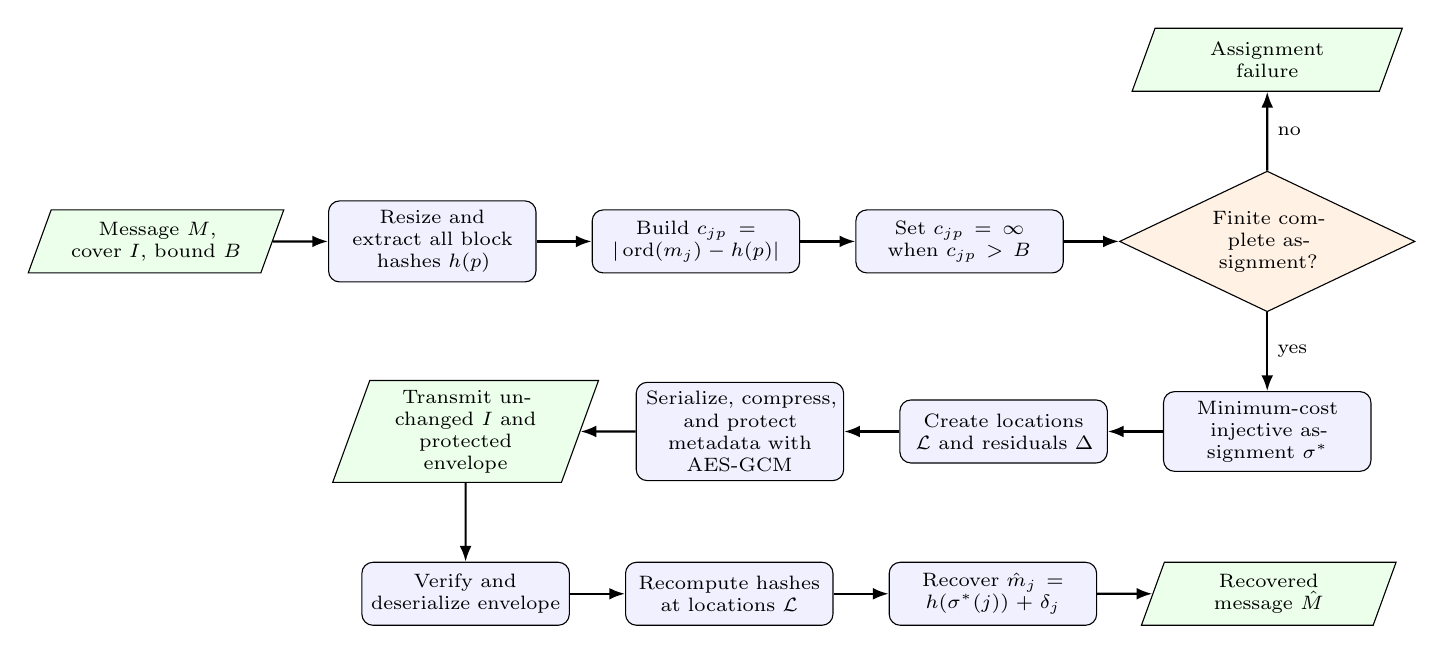
\begin{tikzpicture}[
    node distance=5mm and 7mm,
    font=\scriptsize,
    process/.style={
        rectangle,
        rounded corners,
        draw=black,
        align=center,
        minimum height=8mm,
        text width=24mm,
        fill=blue!6
    },
    decision/.style={
        diamond,
        aspect=2.1,
        draw=black,
        align=center,
        inner sep=1pt,
        text width=19mm,
        fill=orange!10
    },
    data/.style={
        trapezium,
        trapezium left angle=70,
        trapezium right angle=110,
        draw=black,
        align=center,
        minimum height=8mm,
        text width=22mm,
        fill=green!8
    },
    arrow/.style={-{Latex[length=2mm]}, thick}
]
\node[data] (inputs) {Message $M$, cover $I$, bound $B$};
\node[process, right=of inputs] (hash) {Resize and extract all block hashes $h(p)$};
\node[process, right=of hash] (cost) {Build $c_{jp}=|\operatorname{ord}(m_j)-h(p)|$};
\node[process, right=of cost] (mask) {Set $c_{jp}=\infty$ when $c_{jp}>B$};
\node[decision, right=of mask] (feasible) {Finite complete assignment?};

\node[process, below=10mm of feasible] (assign) {Minimum-cost injective assignment $\sigma^*$};
\node[process, left=of assign] (records) {Create locations $\mathcal L$ and residuals $\Delta$};
\node[process, left=of records] (protect) {Serialize, compress, and protect metadata with AES-GCM};
\node[data, left=of protect] (send) {Transmit unchanged $I$ and protected envelope};

\node[process, below=10mm of send] (verify) {Verify and deserialize envelope};
\node[process, right=of verify] (rehash) {Recompute hashes at locations $\mathcal L$};
\node[process, right=of rehash] (recover) {Recover $\hat m_j=h(\sigma^*(j))+\delta_j$};
\node[data, right=of recover] (output) {Recovered message $\hat M$};
\node[data, above=10mm of feasible] (failure) {Assignment failure};

\draw[arrow] (inputs) -- (hash);
\draw[arrow] (hash) -- (cost);
\draw[arrow] (cost) -- (mask);
\draw[arrow] (mask) -- (feasible);
\draw[arrow] (feasible) -- node[right]{yes} (assign);
\draw[arrow] (feasible) -- node[right]{no} (failure);
\draw[arrow] (assign) -- (records);
\draw[arrow] (records) -- (protect);
\draw[arrow] (protect) -- (send);
\draw[arrow] (send) -- (verify);
\draw[arrow] (verify) -- (rehash);
\draw[arrow] (rehash) -- (recover);
\draw[arrow] (recover) -- (output);
\end{tikzpicture}%
}
\caption{FHAM assignment and reconstruction workflow. The formal contribution is the bounded location assignment; transport of the authenticated records is outside the evaluated protocol scope.}
\label{fig:fham_workflow}
\end{figure*}

\subsection{Hash Code Generation}

The cover image $I$ is resized to $512 \times 512$ and partitioned into
non-overlapping $24\times24$ blocks. Each block is divided into a $3\times3$
grid of $8\times8$ sub-blocks. For sub-block $B_j$, the implementation centers
its intensities and computes the spectral score
\begin{equation}
    e_j=\lambda_{\max}(\widetilde{B}_j\widetilde{B}_j^{\mathsf T}),
    \qquad \widetilde{B}_j=B_j-\operatorname{mean}(B_j).
\end{equation}
Four 8-bit hashes are then produced. Three compare consecutive scores along
zigzag, row-wise, and column-wise traversals; the fourth compares the center
score with the eight surrounding scores. Each block therefore contributes four
locations $(x,y,k)$ with hash values in $\{0,\ldots,255\}$. For a
$512\times512$ image, the $21\times21$ complete blocks yield
$21^2\times4=1764$ locations.

\subsection{Minimum-Displacement Assignment Algorithm}

FHAM performs a global assignment over all message symbols and all available
locations:

\begin{algorithm}[!t]
    \caption{FHAM Bounded Intra-Cover Assignment}
    \label{alg:embed}
    \begin{algorithmic}[1]
        \Require Secret message $M$, cover image $I$, bound $B$
        \Ensure Location sequence $\mathcal{L}$, displacement sequence $\Delta$
        \State $\mathcal{L} \gets []$, $\Delta \gets []$
        \State Build lookup table $\mathcal{T}$ from $I$
        \State $N(I) \gets \sum_{a \in \mathrm{keys}(\mathcal{T})} |\mathcal{T}(a)|$
        \If{$|M| > N(I)$}
            \State \Return failure
        \EndIf
        \State Enumerate locations $\mathcal{P}(I)=\{p_1,\ldots,p_N\}$
        \State $c_{jp}\gets|\text{ord}(m_j)-h(p)|$
        \State Set $c_{jp}\gets\infty$ wherever $c_{jp}>B$
        \State $\sigma^*\gets\textsc{LinearAssignment}([c_{jp}])$
        \If{no finite complete assignment exists}
            \State \Return failure
        \EndIf
        \For{$j=1$ to $|M|$}
            \State Append $\sigma^*(j)$ to $\mathcal{L}$
            \State Append $\text{ord}(m_j)-h(\sigma^*(j))$ to $\Delta$
        \EndFor
        \State \Return $\mathcal{L},\Delta$
    \end{algorithmic}
\end{algorithm}

\begin{proposition}[Algorithmic Correctness]
Algorithm~\ref{alg:embed} returns a valid assignment if and only if the cost
matrix contains a finite complete assignment. When it succeeds,
$|\delta_j|\leq B$ for every symbol and its total $L_1$ cost is minimum among
all assignments satisfying the same bound.
\end{proposition}

\subsection{Extraction}

Bob receives $I$, $\mathcal{L}$, and $\Delta$ through the chosen communication
layer and reconstructs each character:
\begin{equation}
    \hat{m}_j = \operatorname{chr}\!\left(
    h(x_j,y_j,k_j;I)+\delta_j\right),
\end{equation}
where $h(x_j,y_j,k_j;I)$ recomputes arrangement $k_j$ on the block
$I[y_j:y_j+L,\;x_j:x_j+L]$. The authenticated auxiliary envelope is verified
before deserialization and extraction.

\section{Experimental Results}
\label{sec:experiments}

\subsection{Experimental Setup}

The controlled experiments use the eight scikit-image covers shown in
Fig.~\ref{fig:cover_images}, converted to grayscale and resized to
$512\times512$. For each cover and message length, ten printable-ASCII messages
are generated from deterministic seeds. Capacity is evaluated at lengths
$10,20,30,40,50,60,80,100,150,$ and $200$, for a total of 800 trials.
Assignment and channel experiments use the stated subsets of these lengths and
the same ten-message protocol. A separate stress corpus contains 19
heterogeneous scikit-image references and 200 LFW face thumbnails, all resized
to $512\times512$; three messages per image and length yield 1314 stress trials.
The bounded stress experiment at length 200 uses one deterministic message per
image, hence 219 trials for each value of $B$.
Exact preprocessed PNG copies and provenance manifests accompany the
implementation under \texttt{dataset/controlled} and \texttt{dataset/stress}.
The corpus contains photographs,
scientific images, LFW face photographs, scanned documents, and a small number
of explicitly identified graphical reference cases.
The Abdulsattar comparison implements the published strongest-capacity
configuration: $18\times18$ blocks, nine $6\times6$ sub-blocks, Arr.4
eigenvalue comparisons, six-pixel stride, exact ASCII matching, and no
location reuse \cite{abdulsattar2021}. The WYSAWIS comparison implements the
published $4\times4$ raster hash, zero-count categories, first useful block per
category, ascending decimal sequence ranks, and 15-bit message segmentation.
A WYSAWIS cover is adequate only if all 16 categories occur. Its Google Drive
transfer is represented through the published counts of selected cloud files
and required cover-file corpus.
Measurements were obtained with Python 3.13.5
on Windows 10 using an Intel Core i7-10850H CPU; NumPy 2.2.6 and SciPy 1.17.1
provide the numerical and assignment routines. Reported times are wall-clock
means and are reported as implementation-specific measurements.
The evaluation covers dense-versus-aggregated formulation equivalence, an
extended assignment ablation (exact matching, bottleneck, and
random-feasible baselines), a five-point stability-aware $\lambda$ sweep with
disjoint development and validation transformation subsets, a causal ablation
crossing four codebooks with the same assignment strategies, a
descriptor-family comparison followed by a validation-gated selection on a
BOSSBase sample, the complete four-family eight-length message manifest, a
message-length leakage measurement for the protected envelope, an
H0/H1 traffic-detectability check with four classifiers, a 36-condition
extended transformation matrix, and, on external samples, a 180-image check
across BOSSBase, BOWS2, and COCO~2017 together with a larger stratified
robustness check on the same three corpora. Reproduction details, complete protocol notes, and additional evidence are provided in Supplementary Material S1; the self-contained code/results artefact is Supplementary Material S2.

\subsection{Metrics and Terminology}
\label{sec:metrics}

We use \emph{assignment feasibility} for the event that the solver finds an
injective message-to-location assignment on the original, preprocessed cover
such that every residual satisfies the stated bound. The Assignment Success
Rate (ASR) is the fraction of tested cover--message pairs for which this event
occurs. ASR quantifies the original-cover assignment condition. The separately
reported exact recovery rate quantifies complete post-transformation message
reconstruction, so the two metrics describe distinct stages of the system.

We use \emph{exact recovery rate} for the fraction of trials in which the full
reconstructed message equals the original message after the specified
transformation or channel operation. Character accuracy is the fraction of
individual symbols reconstructed correctly, averaged over the tested
messages. These metrics are reported separately because a message can be
feasible to assign on the original cover while its exact recovery depends on
the transformed cover and channel. Unless stated otherwise, lengths in byte-oriented message-family
experiments are bytes; controlled printable-ASCII experiments may equivalently
describe these lengths as characters because each tested character is one
byte.

\begin{figure*}[!t]
\centering
\begin{subfigure}{0.22\textwidth}
    \centering
    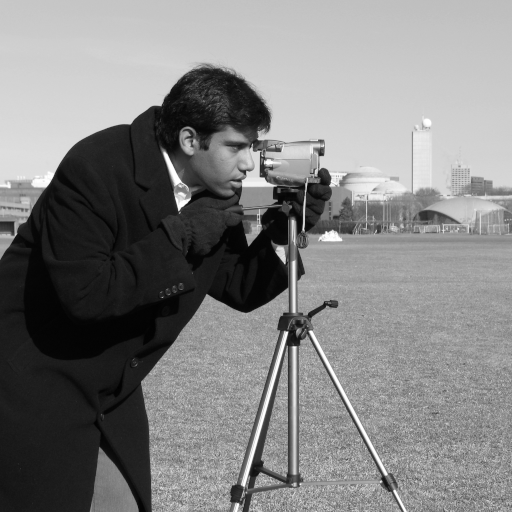
\includegraphics[width=\linewidth]{camera.png}
    \caption{Camera}
\end{subfigure}
\hfill
\begin{subfigure}{0.22\textwidth}
    \centering
    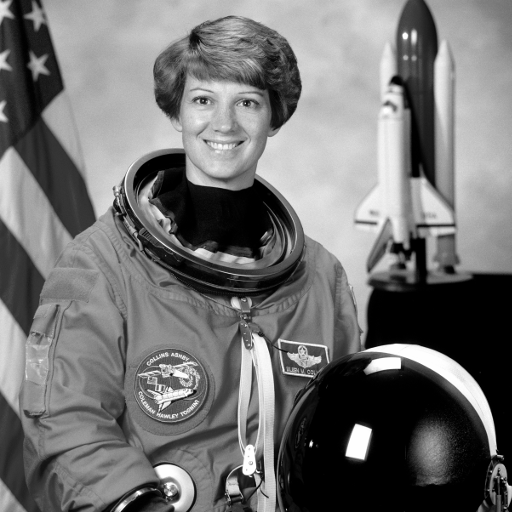
\includegraphics[width=\linewidth]{astronaut.png}
    \caption{Astronaut}
\end{subfigure}
\hfill
\begin{subfigure}{0.22\textwidth}
    \centering
    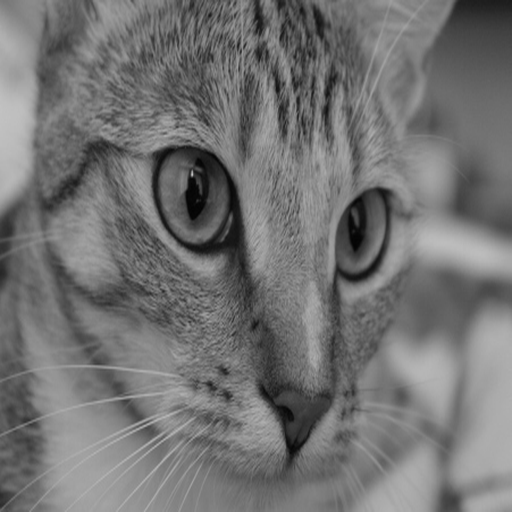
\includegraphics[width=\linewidth]{chelsea.png}
    \caption{Chelsea}
\end{subfigure}
\hfill
\begin{subfigure}{0.22\textwidth}
    \centering
    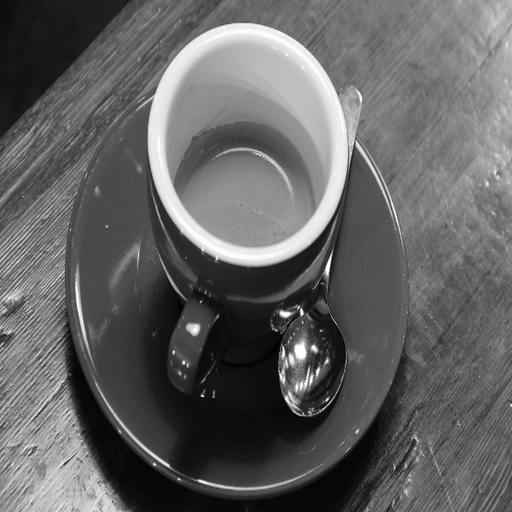
\includegraphics[width=\linewidth]{coffee.png}
    \caption{Coffee}
\end{subfigure}

\vspace{0.5cm}

\begin{subfigure}{0.22\textwidth}
    \centering
    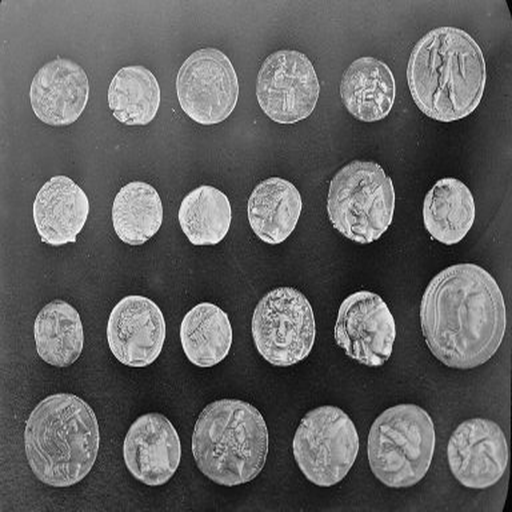
\includegraphics[width=\linewidth]{coins.png}
    \caption{Coins}
\end{subfigure}
\hfill
\begin{subfigure}{0.22\textwidth}
    \centering
    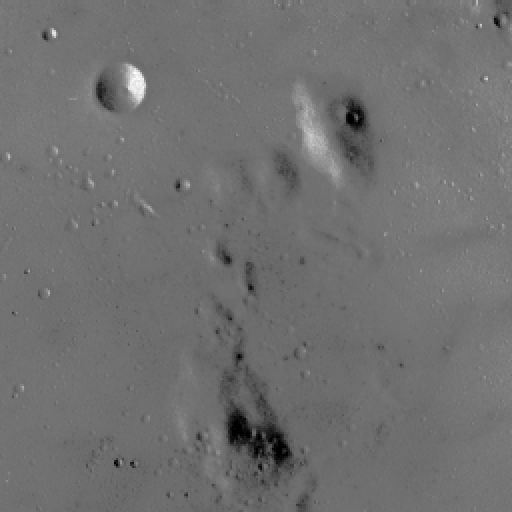
\includegraphics[width=\linewidth]{moon.png}
    \caption{Moon}
\end{subfigure}
\hfill
\begin{subfigure}{0.22\textwidth}
    \centering
    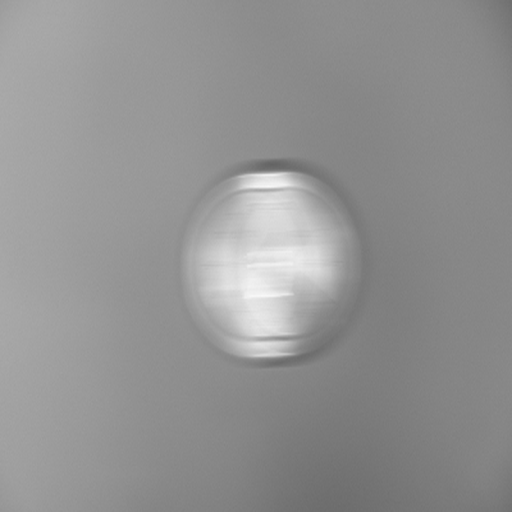
\includegraphics[width=\linewidth]{clock.png}
    \caption{Clock}
\end{subfigure}
\hfill
\begin{subfigure}{0.22\textwidth}
    \centering
    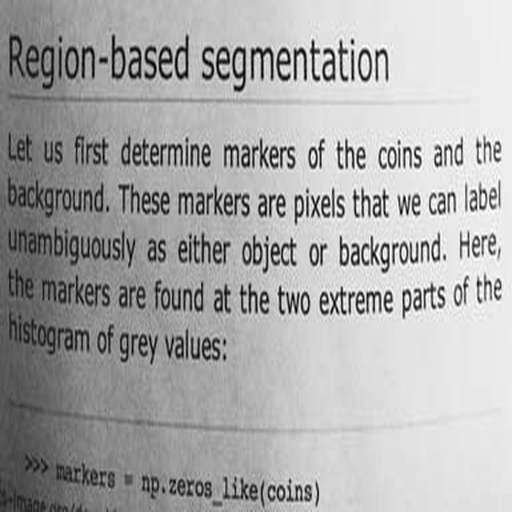
\includegraphics[width=\linewidth]{page.png}
    \caption{Page}
\end{subfigure}
\caption{Standard test images used in the experiments.}
\label{fig:cover_images}
\end{figure*}
\subsection{Capacity Analysis}

Fig.~\ref{fig:capacity} compares the Assignment Success Rate (ASR) as a function
of message length over eight images and ten trials per image. The exact-match
baseline decreases from 86.25\% at 10 characters to 0\% at 150 and 200
characters. Bounded FHAM with $B=2$ achieves 100\% ASR at every tested length
from 10 to 200 characters. Each image provides 1764 distinct locations under
the $24\times24$ non-overlapping block configuration.

\begin{figure}[!t]
    \centering
    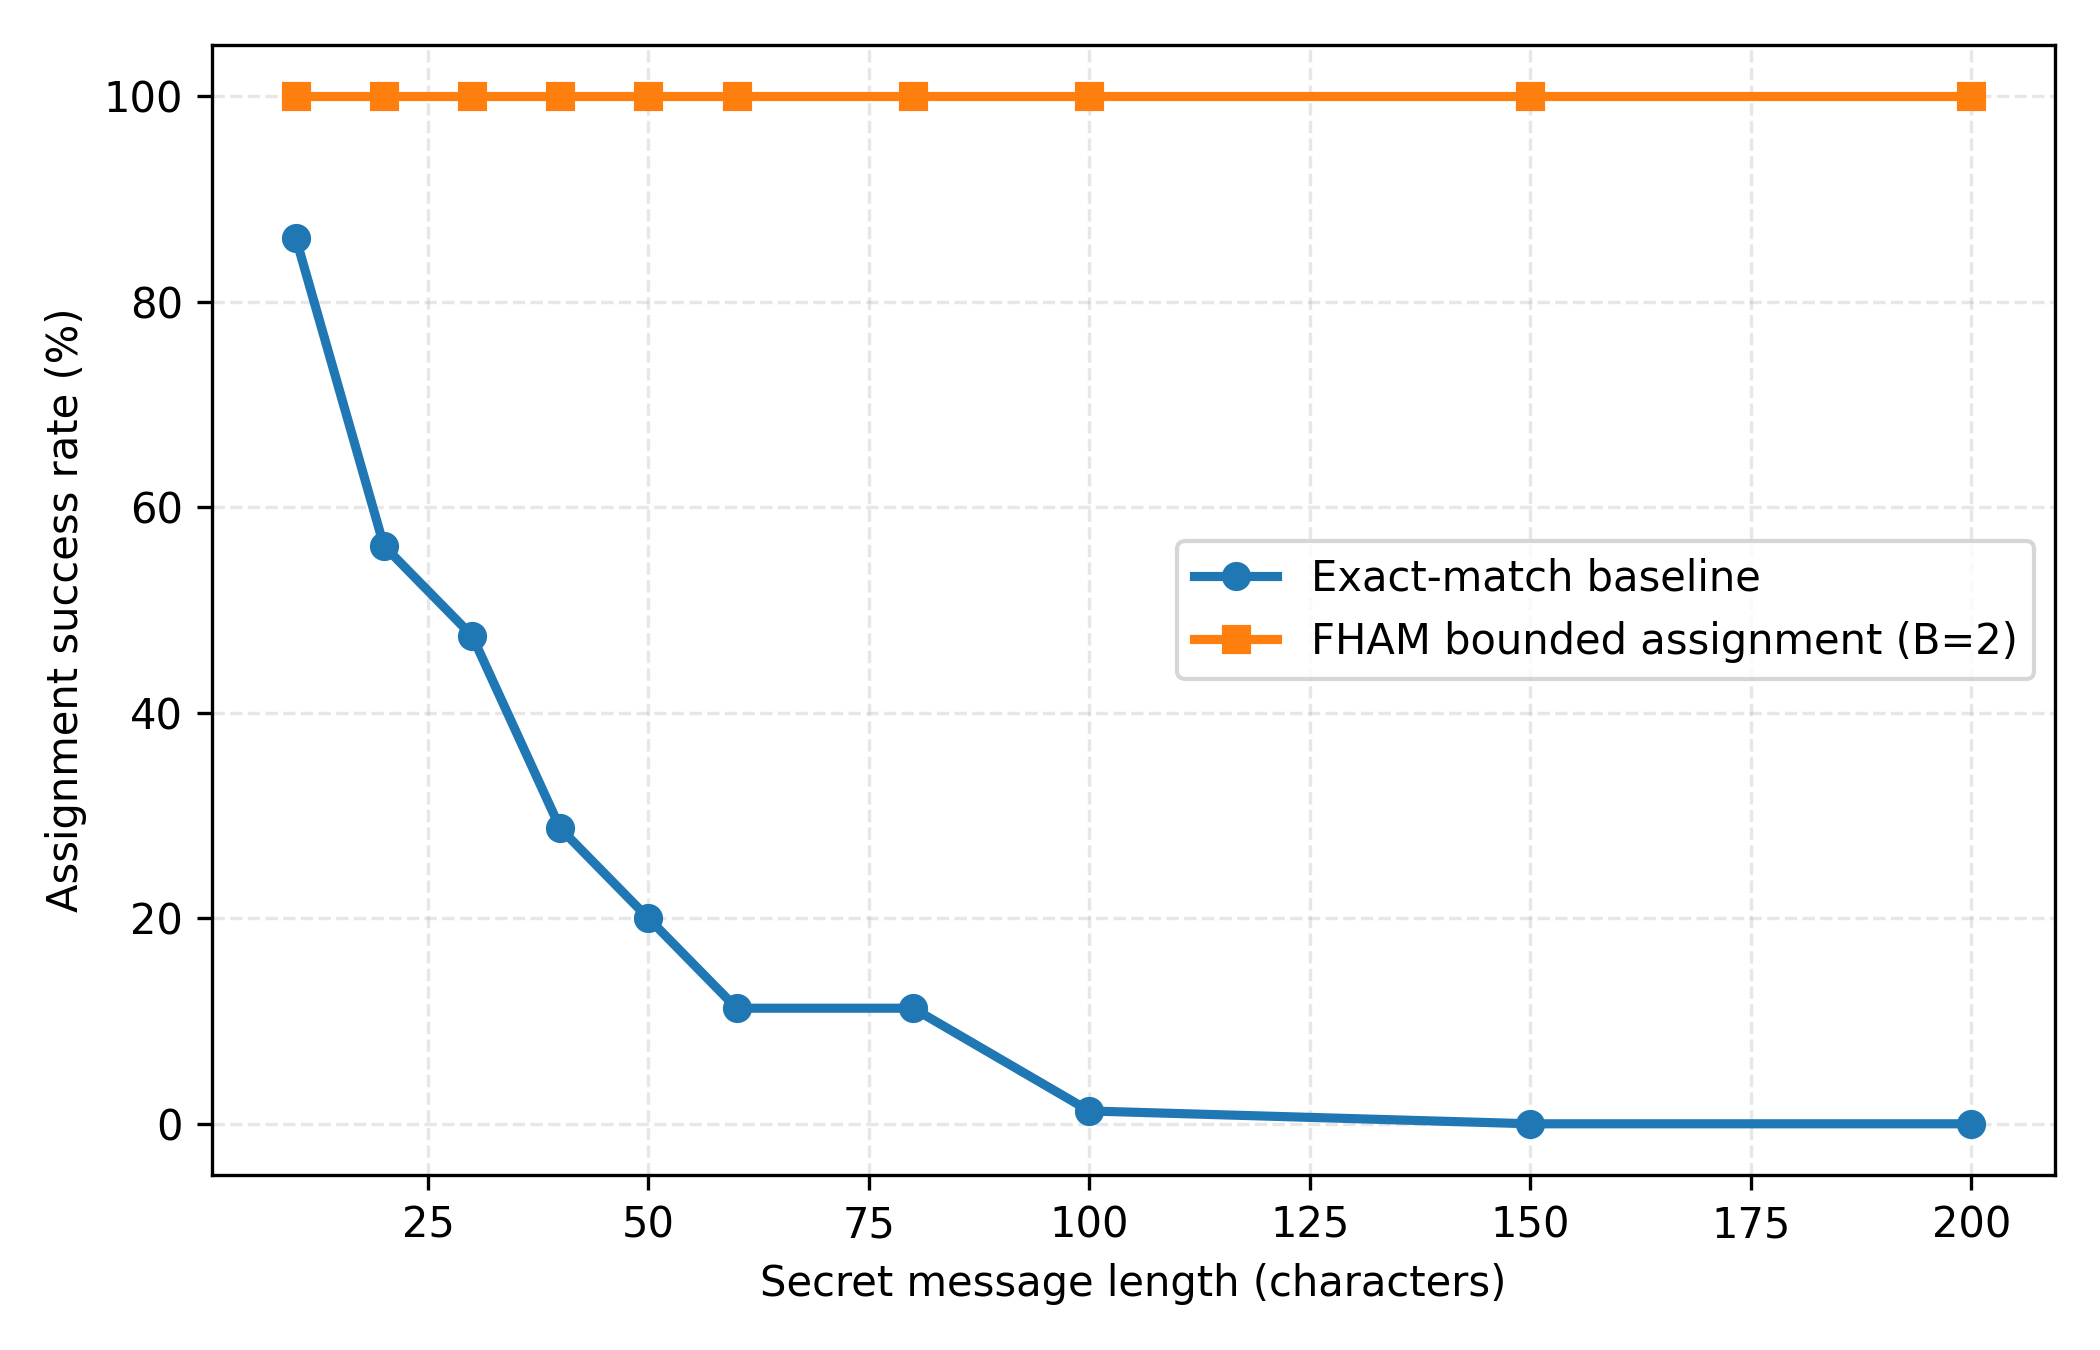
\includegraphics[width=\linewidth]{fig_capacity.png}
\caption{Assignment feasibility rate on the eight-image controlled set. Bounded FHAM uses $B=2$. Feasibility is evaluated on the original cover before channel transformations.}
    \label{fig:capacity}
\end{figure}

\subsection{Direct Comparison with Abdulsattar and WYSAWIS}

Table~\ref{tab:mapping_comparison} reports all three methods on identical
as-given covers and messages. At 200 characters, FHAM succeeds on all
controlled covers and on 163/219 stress covers. Abdulsattar's overlapping
variant succeeds on 0/8 controlled covers and 1/219 stress covers. Its 6889
locations are numerous, while exact encoding remains governed by the
multiplicity of each required ASCII code. WYSAWIS succeeds on 3/8 controlled covers and
111/219 stress covers because only these covers contain all 16 categories.
These rates answer a fixed-cover question; WYSAWIS can instead search a shared
database for an adequate cover.

\begin{table*}[!t]
\centering
\caption{Three-Way Comparison Under a Common Fixed-Cover Protocol}
\label{tab:mapping_comparison}
\resizebox{\linewidth}{!}{%
\begin{tabular}{
  >{\raggedright\arraybackslash}p{3.6cm}
  >{\raggedleft\arraybackslash}p{2.6cm}
  >{\raggedleft\arraybackslash}p{2.6cm}
  >{\raggedleft\arraybackslash}p{3.0cm}
}
\toprule
\textbf{Metric at 200 characters} & \textbf{FHAM ($B=2$)} &
\textbf{Abdulsattar Arr.4} & \textbf{WYSAWIS core} \\
\midrule
Controlled as-given cover assignment feasibility & 100.0\% & 0.0\% & 37.5\% \\
Stress as-given cover assignment feasibility & 74.4\% & 0.46\% & 50.7\% \\
Identity recovery when mapping exists & 100.0\% & 100.0\% & 100.0\% \\
Per-message representation records & 200 & 200 & 108 \\
Operational side information & Protected locations/residuals & Location table & Cloud file identities \\
Pre-provisioned external corpus & None & None & At least 102,960 files \\
Published nominal capacity & 14,112 bits & 55,112 bits & 491,520 bits \\
\bottomrule
\end{tabular}%
}
\end{table*}

The nominal capacities follow distinct resource models. FHAM's value is its
number of distinct hash locations times eight, with bounded feasibility
characterized by Hall's condition. Abdulsattar's value similarly counts
overlapping locations, while effective success depends on exact hash
multiplicity. WYSAWIS derives its value from the 15-bit sequence space and
permits repeated representation through distinct cloud files. At 200
characters, its 108 location identities have a mean information-theoretic
lower bound of 1793 bits on the stress corpus. FHAM's reported 549.4-byte
figure includes measured serialization, compression, nonce, and
authentication; the other columns use their respective published operational
units.

\subsection{Greedy Versus Global Assignment}

Table~\ref{tab:assignment_ablation} compares the capacity-aware greedy rule
with the global linear assignment over eight images and ten messages per image.
At short lengths the two methods coincide because almost every printable target
has an unused exact-match location. At 100 and 200 characters, global
assignment reduces total displacement. A paired one-sided Wilcoxon test gives
$p=0.0156$ at length 100 and $p<10^{-13}$ at length 200; the methods coincide
at shorter lengths. The SciPy implementation is also faster
than the Python greedy loop for the tested sizes; this is an implementation
result rather than an asymptotic claim.

\begin{table*}[!t]
\centering
\caption{Assignment Ablation: Mean Total Displacement and Assignment Time}
\label{tab:assignment_ablation}
\begin{tabular}{rrrrr}
\toprule
\textbf{Length} & \textbf{Greedy $D_1$} & \textbf{Global $D_1$} & \textbf{Greedy (ms)} & \textbf{Global (ms)} \\
\midrule
20 & 0.56 & 0.56 & 1.32 & 0.70 \\
50 & 1.98 & 1.91 & 3.14 & 1.24 \\
100 & 5.94 & 5.74 & 6.63 & 2.91 \\
200 & 26.31 & 23.73 & 12.82 & 4.74 \\
\bottomrule
\end{tabular}

\end{table*}

\subsection{Dense Versus Aggregated Flow Formulation}

Section~\ref{sec:formal_model} develops both a dense symbol-position cost
matrix and an aggregated formulation over the 256 possible hash values,
solved respectively by rectangular linear assignment and by a min-cost-flow
solver over demand/capacity nodes. Table~\ref{tab:formulation_comparison}
checks this equivalence empirically: for every one of the 160 trials in which
at least one formulation is feasible, the two solvers agree on feasibility
and report an identical optimal cost (100\% cost agreement at every tested
length). The dense solver, implemented with SciPy's rectangular
Jonker--Volgenant routine, is one to two orders of magnitude faster in wall
clock time than the pure-Python shortest-successive-paths implementation of
the aggregated min-cost flow used in this study; as with the greedy-versus-global
timing in Table~\ref{tab:assignment_ablation}, this is an implementation
result for the two solvers compared here and not an asymptotic claim about
the two formulations in general.

\begin{table}[!t]
\centering
\caption{Dense Versus Aggregated Flow: Cost Agreement and Running Time}
\label{tab:formulation_comparison}
\begin{tabular}{rrrrr}
\toprule
\textbf{Length} & \textbf{Feasible} & \textbf{Cost Agree.} & \textbf{Dense (ms)} & \textbf{Aggreg. (ms)} \\
\midrule
50 & 100.0\% & 100.0\% & 0.81 & 14.97 \\
100 & 100.0\% & 100.0\% & 2.34 & 35.49 \\
200 & 100.0\% & 100.0\% & 4.38 & 60.18 \\
400 & 55.0\% & 100.0\% & 10.06 & 82.67 \\
\bottomrule
\end{tabular}

\end{table}

\subsection{Extended Assignment Ablation}

Table~\ref{tab:extended_ablation} extends the greedy-versus-global comparison
with four further baselines evaluated on the identical spectral codebook and
$B=2$: unbounded exact matching (A1, the zero-residual reference), minimum-bottleneck
assignment (A4, minimizing the maximum $|\delta|$ by binary search over the
threshold before solving a feasibility-checked rectangular assignment), a
randomized feasible assignment (A6, a heuristic lower-anchor baseline that
scans targets in a fixed order and draws a uniformly random feasible location
at each step), and the stability-aware cost at its frozen $\lambda=0.75$
(Section~\ref{sec:experiments}). Exact matching fails almost immediately, confirming the
motivation for bounded assignment: only 20.0\% and 1.25\% of trials succeed at
50 and 100 bytes, and none at 200. Bottleneck assignment keeps the maximum
displacement close to $B$ while its total displacement tracks the $L_1$-optimal
global assignment closely. Random feasible assignment always saturates the
bound (mean maximum $|\delta|=2=B$) and its total displacement is 3 to 10
times higher than the optimal assignment; it also becomes infeasible on 5\% of
trials at 200 bytes even though global\_l1 finds a feasible assignment on the
same instances, which is expected of an unordered random heuristic and is
reported as a naive lower-anchor baseline for context.
Stability-aware assignment at $B=2$ always succeeds but at a higher total
displacement than global $L_1$ (e.g., 90.56 versus 23.73 at 200 bytes), the
expected cost of also weighting transformation stability in the cost
function rather than residual size alone.

\begin{table*}[!t]
\centering
\caption{Extended Assignment Ablation at $B=2$}
\label{tab:extended_ablation}
\resizebox{\linewidth}{!}{\begin{tabular}{lrrrrr}
\toprule
\textbf{Method} & \textbf{Length} & \textbf{Success} & \textbf{Mean $D_1$} & \textbf{Mean Max $|\delta|$} & \textbf{Time (ms)} \\
\midrule
Exact matching (A1) & 50 & 20.00\% & 0.00 & 0.00 & 0.10 \\
Exact matching (A1) & 100 & 1.25\% & 0.00 & 0.00 & 0.11 \\
Exact matching (A1) & 200 & 0.00\% & -- & -- & 0.10 \\
Greedy & 50 & 100.00\% & 1.98 & 0.81 & 2.68 \\
Greedy & 100 & 100.00\% & 5.94 & 1.14 & 5.51 \\
Greedy & 200 & 100.00\% & 26.31 & 2.11 & 10.60 \\
Global $L_1$ & 50 & 100.00\% & 1.91 & 0.81 & 1.32 \\
Global $L_1$ & 100 & 100.00\% & 5.74 & 1.14 & 2.68 \\
Global $L_1$ & 200 & 100.00\% & 23.73 & 1.76 & 4.76 \\
Bottleneck (A4) & 50 & 100.00\% & 1.91 & 0.80 & 1.70 \\
Bottleneck (A4) & 100 & 100.00\% & 5.74 & 1.01 & 4.37 \\
Bottleneck (A4) & 200 & 100.00\% & 23.76 & 1.25 & 8.53 \\
Random feasible (A6) & 50 & 100.00\% & 62.71 & 2.00 & 5.70 \\
Random feasible (A6) & 100 & 100.00\% & 121.19 & 2.00 & 11.12 \\
Random feasible (A6) & 200 & 95.00\% & 248.29 & 2.00 & 21.06 \\
Stability-aware & 50 & 100.00\% & 13.51 & 1.52 & 25.23 \\
Stability-aware & 100 & 100.00\% & 30.23 & 1.84 & 51.38 \\
Stability-aware & 200 & 100.00\% & 90.56 & 2.00 & 99.94 \\
\bottomrule
\end{tabular}
}
\end{table*}

\subsection{Stability-Aware Cost and Lambda Selection}

The stability-aware cost $c=\lambda\cdot\text{normalized\_residual}+(1-\lambda)\cdot(1-\text{stability})$
is swept over $\lambda\in\{0,0.25,0.5,0.75,1\}$ at $B=8$, length 100, on the
eight controlled images. Per-location stability is estimated as the fraction
of a three-transform \emph{development} subset (JPEG quality 90, downscale-restore
0.9, Gaussian noise $\sigma=1$) under which a location's descriptor hash is
unchanged from the identity cover. Recovery is then measured under three
disjoint \emph{validation} transformations (JPEG quality 75, $1^\circ$ rotation,
Gaussian noise $\sigma=2$), keeping validation measurements independent of
the stability estimate. Table~\ref{tab:stability_lambda} reports every tested
$\lambda$. All five values reach 100\% assignment feasibility; exact recovery
is 0\% under the validation channel. Weighting toward stability
($\lambda\leq0.75$) raises character accuracy from 33.8\% at $\lambda=1$
(pure residual minimization, equivalent to global $L_1$) to 55.1--55.4\%.
The highest observed character accuracy is 55.4\% at $\lambda=0$, with mean
total displacement 731.98; $\lambda=0.75$ gives 55.1\% with displacement
50.77. We use $\lambda=0.75$ as a practical accuracy--displacement operating
point in the remaining experiments. These validation values informed the
selection and therefore serve as tuning results rather than an independent
estimate of generalization. The sweep shows that stability weighting can
substantially reduce displacement relative to $\lambda=0$ while retaining
character accuracy near the best observed value; exact recovery remains 0\%
under this channel.

We assessed transfer of this operating region on 11 non-face stress images,
using three 200-byte templated messages per image, zlib preprocessing, the
spectral $12\times12$ profile, and $B=2$. Stability was estimated on the same
development transformations and evaluated on the disjoint JPEG~75, rotation,
and noise~2 conditions. Each $\lambda$ produced a feasible assignment for 32
of 33 image--message cases. Values $0.25$, $0.5$, and $0.75$ produced the same
mean displacement (21.97) and closely matched byte accuracies (57.8\% for
JPEG~75, 68.1\% for noise, and 9.4\% for rotation). At $\lambda=0$, mean
displacement rose to 211.47 with slightly lower accuracy; at $\lambda=1$,
displacement fell to 2.78 while accuracy fell to 29.2\%, 38.1\%, and 3.8\%.
Exact recovery of the source message remained 0/99 for every weight. This
external check supports the mid-range accuracy--displacement trade-off on the
sampled images and messages; its 11-image size does not establish a universal
weight or generalization to other channel distributions.

\begin{table}[!t]
\centering
\caption{Stability-Aware Lambda Sweep ($B=8$, Length 100)}
\label{tab:stability_lambda}
\begin{tabular}{rrrrr}
\toprule
$\boldsymbol{\lambda}$ & \textbf{Success} & \textbf{Mean $D_1$} & \textbf{Validation Exact} & \textbf{Validation Acc.} \\
\midrule
0.00 & 100.0\% & 731.98 & 0.0\% & 55.4\% \\
0.25 & 100.0\% & 54.77 & 0.0\% & 55.1\% \\
0.50 & 100.0\% & 54.77 & 0.0\% & 55.1\% \\
0.75 & 100.0\% & 50.77 & 0.0\% & 55.1\% \\
1.00 & 100.0\% & 5.42 & 0.0\% & 33.8\% \\
\bottomrule
\end{tabular}

\end{table}

\begin{table}[!t]
\centering
\small
\caption{Transfer of the Stability Weight to the Scene Holdout}
\label{tab:lambda_transfer}
\resizebox{\linewidth}{!}{\begin{tabular}{rrrrrrr}
\toprule
\textbf{$\lambda$} & \textbf{Assignment / 33} & \textbf{Mean $D_1$} & \textbf{JPEG 75 accuracy} & \textbf{Noise $\sigma=2$ accuracy} & \textbf{Rotation $1^\circ$ accuracy} & \textbf{Exact source / 99} \\
\midrule
0.00 & 32 & 211.47 & 57.3\% & 67.4\% & 9.5\% & 0 \\
0.25 & 32 & 21.97 & 57.8\% & 68.1\% & 9.4\% & 0 \\
0.50 & 32 & 21.97 & 57.8\% & 68.1\% & 9.4\% & 0 \\
0.75 & 32 & 21.97 & 57.8\% & 68.1\% & 9.4\% & 0 \\
1.00 & 32 & 2.78 & 29.2\% & 38.1\% & 3.8\% & 0 \\
\bottomrule
\end{tabular}
}
\end{table}

\subsection{Causal Codebook Ablation}

The comparisons above change both the descriptor and the assignment rule at
once when contrasting FHAM with Abdulsattar. Table~\ref{tab:causal_ablation}
isolates these two factors by crossing four codebooks (D0 spectral, D1
DCT-ordinal, D2 wavelet-gradient, and Abdulsattar's own Arr.4 codebook) with
the same assignment strategies on the same eight images and 200-byte
messages (80 trials per cell): exact matching, bounded global $L_1$ at
$B=2$, unbounded global $L_1$, and the frozen stability-aware cost
($\lambda=0.75$) where a compatible transformation-based stability estimate
exists. FHAM's bounded and global solvers require only a value-to-locations
lookup table, so they are applied to Abdulsattar's codebook without
modifying it; Abdulsattar's published protocol already performs exact
matching, so its exact-matching row is its original protocol under this
common evaluation. Exact matching fails on \emph{every} codebook at this
length, including Abdulsattar's own: 0\% success on all four. Switching only
the assignment rule, holding the codebook fixed, raises success to
92.5--100\% on all four codebooks. This directly attributes FHAM's gain over
Abdulsattar to the bounded/global assignment rule rather than to a
simultaneous change of descriptor. A further, unanticipated observation is
that Abdulsattar's codebook combined with FHAM's bounded solver reaches 100\%
success at a substantially lower mean total displacement (6.3) than any of
the three FHAM descriptors (23.7--40.5) at the same bound; the two
contributions are therefore complementary rather than redundant, and
combining Abdulsattar's descriptor with FHAM's assignment layer is a natural
direction for subsequent study. Stability-aware assignment requires a
stability estimate obtained by
re-hashing a location with the same descriptor used to build the codebook,
which is unavailable for Abdulsattar's incompatible hash function; the
corresponding table cell is therefore unreported.

\begin{table}[!t]
\centering
\caption{Causal Codebook Ablation at 200 Bytes (80 Trials per Cell)}
\label{tab:causal_ablation}
\begin{tabular}{llrr}
\toprule
\textbf{Codebook} & \textbf{Strategy} & \textbf{Success} & \textbf{Mean $D_1$} \\
\midrule
Abdulsattar Arr.4 & Exact matching & 0.0\% & -- \\
Abdulsattar Arr.4 & Bounded $L_1$ ($B{=}2$) & 100.0\% & 6.30 \\
Abdulsattar Arr.4 & Unbounded global $L_1$ & 100.0\% & 6.30 \\
Spectral (D0) & Exact matching & 0.0\% & -- \\
Spectral (D0) & Bounded $L_1$ ($B{=}2$) & 100.0\% & 23.73 \\
Spectral (D0) & Unbounded global $L_1$ & 100.0\% & 23.73 \\
Spectral (D0) & Stability-aware & 100.0\% & 90.56 \\
DCT ordinal (D1) & Exact matching & 0.0\% & -- \\
DCT ordinal (D1) & Bounded $L_1$ ($B{=}2$) & 98.8\% & 26.82 \\
DCT ordinal (D1) & Unbounded global $L_1$ & 100.0\% & 26.82 \\
DCT ordinal (D1) & Stability-aware & 98.8\% & 101.87 \\
Wavelet-grad. (D2) & Exact matching & 0.0\% & -- \\
Wavelet-grad. (D2) & Bounded $L_1$ ($B{=}2$) & 92.5\% & 34.07 \\
Wavelet-grad. (D2) & Unbounded global $L_1$ & 100.0\% & 40.50 \\
Wavelet-grad. (D2) & Stability-aware & 92.5\% & 100.24 \\
\bottomrule
\end{tabular}

\end{table}

\subsection{Bounded Feasibility and Stress Corpus}

Table~\ref{tab:bounded_stress} separates bounded representability from the
trivial unbounded limit at length 200. On the controlled set, $B=2$ is
sufficient for all 40 trials. On the 219-image stress corpus, the same bound
succeeds for 74.4\% of images (163/219; 95\% Wilson confidence interval:
68.3--79.8\%); success rises monotonically with $B$ and reaches 100\% only in
the unbounded case. This result confirms that capacity depends on hash spacing
and multiplicity rather than location count alone. Fig.~\ref{fig:bounded_assignment}
shows the corresponding controlled-set trend across message lengths.

\begin{table}[!t]
\centering
\caption{Success at 200 Characters Versus Bound}
\label{tab:bounded_stress}
\begin{tabular}{rrr}
\toprule
$B$ & \textbf{Controlled ASR (\%)} & \textbf{Stress ASR (\%)} \\
\midrule
0 & 0.0 & 0.0 \\
1 & 82.5 & 27.9 \\
2 & 100.0 & 74.4 \\
4 & 100.0 & 89.0 \\
8 & 100.0 & 92.7 \\
16 & 100.0 & 96.3 \\
32 & 100.0 & 98.2 \\
64 & 100.0 & 98.6 \\
128 & 100.0 & 99.5 \\
255 & 100.0 & 100.0 \\
\bottomrule
\end{tabular}

\end{table}

\begin{figure}[!t]
\centering
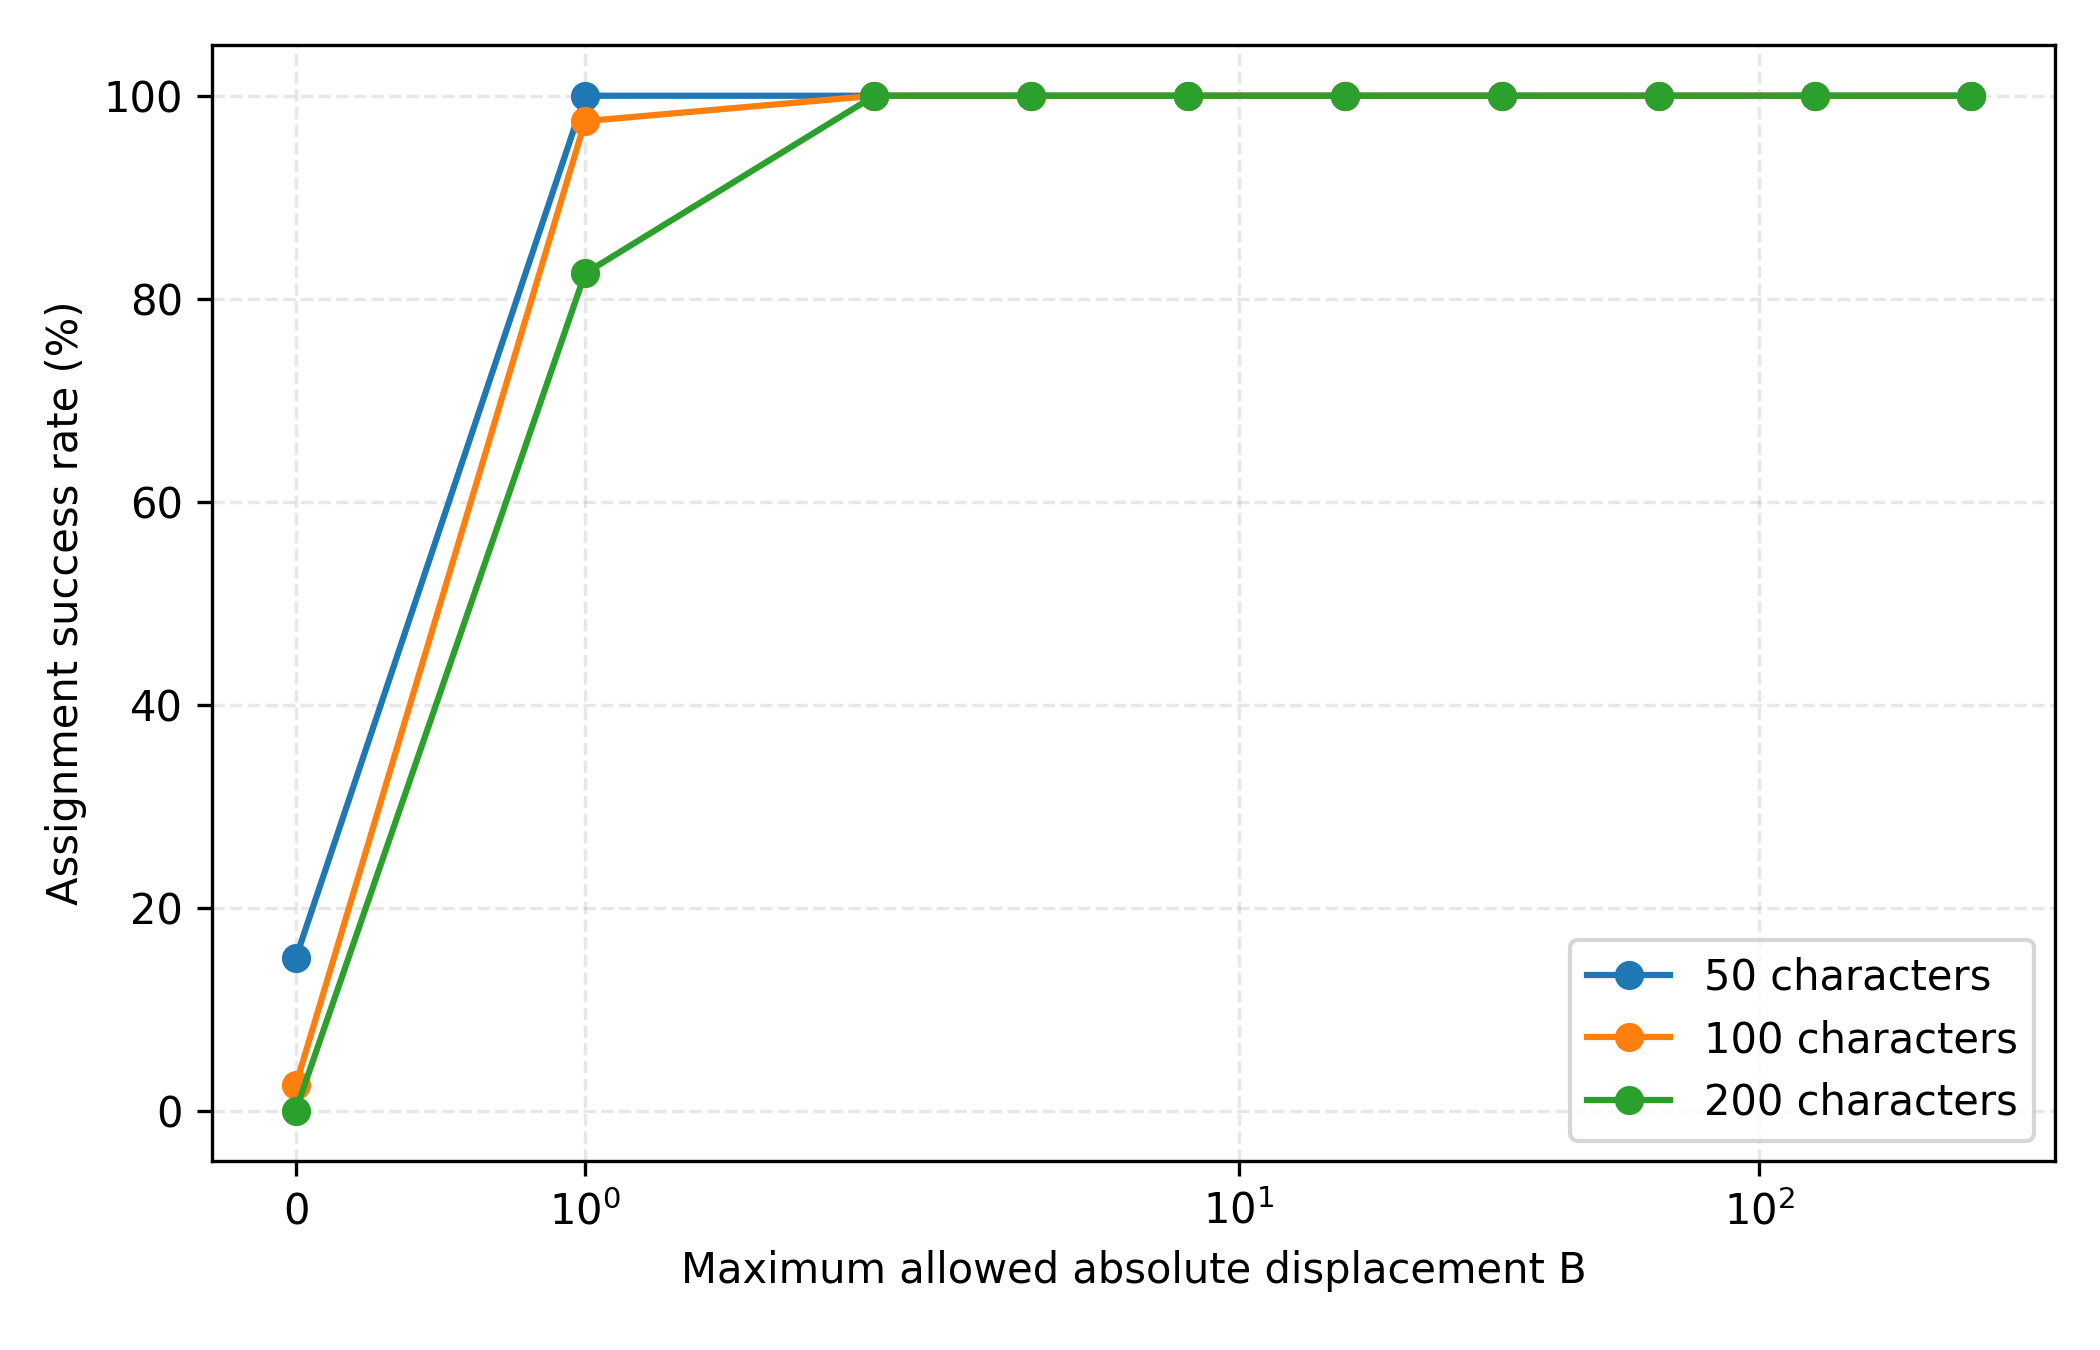
\includegraphics[width=\linewidth]{fig_bounded_assignment.png}
\caption{Controlled-set assignment success as a function of displacement bound.}
\label{fig:bounded_assignment}
\end{figure}

\subsection{Observed Codebook Geometry}

Table~\ref{tab:codebook_geometry} reports the observed codebook geometry. All
images produced 1764 locations and between 247 and 253 distinct hash values.
Despite this variation in density, every codebook had covering radius
$r(\mathcal{A}_I)=1$. Thus, before location depletion, every 8-bit target is
either an exact match or one unit from an available hash. This observation
supports the geometric model for the evaluated dataset and hash construction.

Across the 219-image stress corpus, the median number of distinct hashes is
239 and the median covering radius is 1. However, radii range from 1 to 255:
154 images have radius 1, 45 have radius 2, and the remaining 20 have larger
radii. The degenerate maximum occurs on a near-constant input and explains why
unbounded correction represents a distinct operating regime from
cover-derived capacity.

\begin{table}[!t]
\centering
\caption{Observed Hash-Codebook Geometry}
\label{tab:codebook_geometry}
\begin{tabular}{lrrr}
\toprule
\textbf{Image} & \textbf{Locations} & \textbf{Hashes} & $r(\mathcal{A}_I)$ \\
\midrule
Camera    & 1764 & 253 & 1 \\
Astronaut & 1764 & 253 & 1 \\
Chelsea   & 1764 & 250 & 1 \\
Coffee    & 1764 & 248 & 1 \\
Coins     & 1764 & 253 & 1 \\
Moon      & 1764 & 247 & 1 \\
Clock     & 1764 & 248 & 1 \\
Page      & 1764 & 252 & 1 \\
\bottomrule
\end{tabular}
\end{table}

\subsection{Descriptor Family Comparison}

Section~\ref{sec:methodology} defines three descriptor families sharing the
same $3\times3$ ordinal-comparison construction: the spectral descriptor
(D0) used throughout the rest of this paper, a DCT-ordinal descriptor (D1),
and a wavelet-gradient descriptor (D2). Table~\ref{tab:descriptor_comparison}
evaluates all three under the identical bounded-assignment protocol
($B=2$) rather than reporting only the descriptor actually used elsewhere.
All three produce the same 1764 locations per image (four 8-bit hashes per
$24\times24$ block) but differ in distinct-hash density (mean 250.5, 248.25,
and 243.5 out of 256 for D0, D1, D2) and in codebook-construction time in this
Python implementation (148, 96, and 481~ms). At $B=2$, D0 and D1 reach 100\%
assignment success up to 100 bytes; at 200 bytes D0 remains at 100\%, D1
drops to 98.75\%, and D2 to 92.5\%, with correspondingly higher mean
displacement. Descriptor selection and freezing follow the separate
validation protocol; all three are reported here, including the less favorable D2 result, before
the validation-gated selection performed in the next subsection.

\begin{table*}[!t]
\centering
\caption{Descriptor Family Comparison Under the Bounded Assignment Protocol ($B=2$)}
\label{tab:descriptor_comparison}
\resizebox{\linewidth}{!}{\begin{tabular}{rrrrrrr}
\toprule
& \multicolumn{2}{c}{\textbf{Spectral (D0)}} & \multicolumn{2}{c}{\textbf{DCT Ordinal (D1)}} & \multicolumn{2}{c}{\textbf{Wavelet-Gradient (D2)}} \\
\textbf{Length} & \textbf{Success} & \textbf{Mean $D_1$} & \textbf{Success} & \textbf{Mean $D_1$} & \textbf{Success} & \textbf{Mean $D_1$} \\
\midrule
50 & 100.0\% & 1.91 & 100.0\% & 1.84 & 100.0\% & 3.96 \\
100 & 100.0\% & 5.74 & 100.0\% & 5.64 & 100.0\% & 10.75 \\
200 & 100.0\% & 23.73 & 98.8\% & 26.82 & 92.5\% & 34.07 \\
\bottomrule
\end{tabular}
}
\end{table*}

\subsection{Descriptor Selection on a Validation Sample}

To ground descriptor choice in evidence rather than convention, we evaluate
the three descriptors on 100 images independently drawn from the BOSSBase
validation split (\texttt{dataset/manifests/bossbase.csv}, \texttt{split=validation},
disjoint from the eight controlled images, the 219-image stress corpus, and
the BOSSBase test\_internal/BOWS2/COCO~2017 splits used elsewhere in this
study), at 200 bytes and $B=2$ (\texttt{scripts/select\_descriptor.py}). The
eligibility rule, fixed before evaluation and applied identically to all
three descriptors, requires clean assignment success $\geq99\%$,
median $B^\ast\leq2$, and mean codebook-construction time no more than twice
the spectral descriptor's; ties among eligible descriptors are broken by
higher success, then lower median $B^\ast$, then lower construction time.
Table~\ref{tab:descriptor_selection} reports every candidate, including the
descriptors that fail eligibility. D0 (99.2\% success) and D1 (99.0\% success)
both meet all three criteria; D2 meets only the radius criterion, missing
both the success threshold (87.0\%) and the time threshold (680~ms, more than
twice D0's 183~ms). Applying the tie-break rule to the two eligible
descriptors selects D0 by success rate. This selection is frozen in
\texttt{results/acceptance/frozen\_descriptor.json} before any use of the
BOSSBase test\_internal split, BOWS2, or COCO~2017, and it is consistent with,
rather than a post hoc justification for, the spectral descriptor used as the
default throughout the rest of this study.

\begin{table}[!t]
\centering
\caption{Descriptor Selection on 100 BOSSBase Validation Images (200 Bytes, $B=2$)}
\label{tab:descriptor_selection}
\begin{tabular}{lrrrc}
\toprule
\textbf{Descriptor} & \textbf{Success} & \textbf{Med. $B^\ast$} & \textbf{Build (ms)} & \textbf{Eligible} \\
\midrule
Spectral (D0) & 99.2\% & 1.0 & 182.9 & yes \\
DCT ordinal (D1) & 99.0\% & 1.0 & 131.6 & yes \\
Wavelet-gradient (D2) & 87.0\% & 2.0 & 680.0 & no \\
\bottomrule
\end{tabular}

\end{table}

\subsection{Message Family and Length Coverage}

The experiments above generate printable-ASCII messages from a single ad hoc
seeded generator. Table~\ref{tab:message_family} instead evaluates the full
deterministic message manifest produced by \texttt{scripts/generate\_messages.py}:
four families (uniform random bytes, printable ASCII, templated natural-language text, and
adversarial repeated-byte) at eight byte lengths from 10 to 1600, five
repetitions each, for 40 trials per family-length cell across the eight
controlled images. At $B=2$ the four families diverge sharply in feasible
length. Uniform bytes and printable ASCII, whose symbol values are
comparatively well spread over the codebook, remain fully or mostly feasible
up to 400 bytes and partially so at 800--1200. Templated natural-language text, dominated by a
small set of common ASCII letters from a repeated sentence template, drops to
12.5\% success already at 200 bytes. The adversarial repeated-byte family,
which repeats a single byte value hundreds of times, saturates the
multiplicity of that one hash value almost immediately: 10.0\% at 100 bytes
and 0\% from 200 bytes onward. This confirms, on generated messages rather
than only an informal risk description, that FHAM's effective capacity is
governed by per-symbol multiplicity and message-value distribution, not by
the 1764-location nominal capacity alone.

\begin{table}[!t]
\centering
\caption{Assignment Feasibility Rate by Message Family and Length ($B=2$)}
\label{tab:message_family}
\begin{tabular}{rrrrr}
\toprule
\textbf{Length} & \textbf{Uniform} & \textbf{ASCII} & \textbf{Templated} & \textbf{Adversarial} \\
\midrule
10 & 100.0\% & 100.0\% & 100.0\% & 100.0\% \\
50 & 100.0\% & 100.0\% & 100.0\% & 87.5\% \\
100 & 100.0\% & 100.0\% & 97.5\% & 10.0\% \\
200 & 100.0\% & 100.0\% & 12.5\% & 0.0\% \\
400 & 100.0\% & 75.0\% & 0.0\% & 0.0\% \\
800 & 65.0\% & 0.0\% & 0.0\% & 0.0\% \\
1200 & 5.0\% & 0.0\% & 0.0\% & 0.0\% \\
1600 & 0.0\% & 0.0\% & 0.0\% & 0.0\% \\
\bottomrule
\end{tabular}

\end{table}

\subsection{Pre-assignment Compression and Parameter Ablation}
The message-family results motivate a lossless preprocessing ablation. Before
assignment, each 200-byte source message is either kept unchanged or compressed
with zlib level 9; FHAM then assigns the resulting byte sequence using the same
bounded injective model. After extraction, the receiver decompresses the byte
stream. This preprocessing changes the symbol multiplicities and sequence
length presented to FHAM, while leaving its assignment rule unchanged.

We screened spectral, DCT-ordinal, and wavelet-gradient descriptors over block
sizes 12, 18, 24, 30, 36, and 48 on the eight controlled images. We then
evaluated candidate profiles on 200 LFW face images, using three fixed messages
per family and length (600 image--message cases per cell), and checked the
selected spectral profile on 11 disjoint non-face stress images (33 cases per
cell). The reported $B=2,4,8$ rates are exact feasibility rates determined from
the minimum feasible residual bound. Table~\ref{tab:preprocessing_capacity}
shows the effect of compression for the spectral $12\times12$ profile, which
has 7056 hash locations and a mean codebook-construction time of 428~ms on the
controlled images; the corresponding $24\times24$ profile has 1764 locations
and requires 121~ms. The smaller block profile improves feasibility across
message families, with a higher codebook-construction cost.

On the LFW set, compression changes repeated-byte messages from 200 to 12
bytes and raises $B=2$ feasibility from 0\% to 97.8\%. Templated text changes
from 200 to 116 bytes and rises from 80.5\% to 92.2\%. At $B=4$, the
compressed-message rates reach 98.5\% and 97.2\%, respectively; at $B=8$ they
reach 99.3\% and 98.3\%. The independent scene holdout reports 100\% for
compressed repeated-byte messages and 97.0\% for compressed templated text at
$B=2$. Compression provides little capacity gain for uniform random bytes,
whose compressed length increases to 211 bytes, and printable ASCII, whose
compressed length increases to 201 bytes. These results support compression
for low-entropy inputs and show that block size and $B$ should be selected
against the expected message distribution.

\begin{table}[!t]
\centering
\small
\caption{Lossless Preprocessing and Assignment Feasibility at 200 Source Bytes}
\label{tab:preprocessing_capacity}
\resizebox{\linewidth}{!}{\begin{tabular}{llrrrrr}
\toprule
\textbf{Image subset} & \textbf{Message family} & \textbf{Coded bytes} & \textbf{Uncompressed $B=2$} & \textbf{Compressed $B=2$} & \textbf{Compressed $B=4$} & \textbf{Compressed $B=8$} \\
\midrule
LFW (200 images; 600 cases) & Repeated byte & 12 & 0.0\% & 97.8\% & 98.5\% & 99.3\% \\
LFW (200 images; 600 cases) & Templated text & 116 & 80.5\% & 92.2\% & 97.2\% & 98.3\% \\
LFW (200 images; 600 cases) & Printable ASCII & 201 & 88.3\% & 90.5\% & 96.3\% & 98.0\% \\
LFW (200 images; 600 cases) & Uniform bytes & 211 & 88.7\% & 88.7\% & 97.2\% & 98.0\% \\
Scene holdout (11 images; 33 cases) & Repeated byte & 12 & 57.6\% & 100.0\% & 100.0\% & 100.0\% \\
Scene holdout (11 images; 33 cases) & Templated text & 116 & 90.9\% & 97.0\% & 100.0\% & 100.0\% \\
Scene holdout (11 images; 33 cases) & Printable ASCII & 201 & 90.9\% & 90.9\% & 97.0\% & 100.0\% \\
Scene holdout (11 images; 33 cases) & Uniform bytes & 211 & 90.9\% & 90.9\% & 100.0\% & 100.0\% \\
\bottomrule
\end{tabular}
}
\end{table}

The scene-holdout check confirms transfer of the selected profile across the
sampled image types, while its 11-image size limits the precision of that
estimate. The LFW sweep is a parameter-selection dataset; the scene holdout is
the independent check. The selected profile improves fixed-cover assignment
feasibility and does not alter post-transformation synchronization.

\subsection{Protected Assignment-Record Representation}

The implementation serializes a fixed 15-byte header followed by 4 bytes per
character: a 16-bit token combining block index and arrangement, and a signed
16-bit displacement. We evaluate two protected representations. The compact
representation compresses the serialized payload with zlib level 9 and
protects it using AES-256-GCM. The traffic-shaped representation disables
variable compression, pads the serialized record array to a public fixed
capacity of 200 records, encrypts the padding with the payload, and exposes
only the capacity class. Each envelope adds an authenticated public format
header, a 12-byte random nonce, and a 16-byte authentication tag.
Table~\ref{tab:channel_real} reports protected-envelope size over eight
images and ten messages per length, while Fig.~\ref{fig:auxiliary_channel_real}
shows how the compact serialized, compressed, and encrypted sizes scale. The
direct baseline applies the same compression and authenticated encryption to
the ASCII message alone. Its framing is one format/version byte, a 12-byte
nonce, and the ciphertext with its 16-byte GCM tag, for 29 fixed bytes before
the compressed message. It does not include the 13-byte FHAM record header.
Key establishment is outside these measurements.

\begin{table}[!t]
\centering
\caption{Protected Assignment-Record Cost}
\label{tab:channel_real}
\begin{tabular}{rrrrrr}
\toprule
\textbf{Length} & \textbf{C (B)} & \textbf{S (B)} & \textbf{D (B)} & \textbf{C/D} & \textbf{S/D} \\
\midrule
10 & 94.54 & 852.00 & 47.00 & 2.01 & 18.13 \\
20 & 122.95 & 852.00 & 57.00 & 2.16 & 14.95 \\
50 & 198.99 & 852.00 & 87.00 & 2.29 & 9.79 \\
100 & 314.74 & 852.00 & 137.00 & 2.30 & 6.22 \\
200 & 549.40 & 852.00 & 230.10 & 2.39 & 3.70 \\
\bottomrule
\end{tabular}

\end{table}

\begin{figure}[!t]
\centering
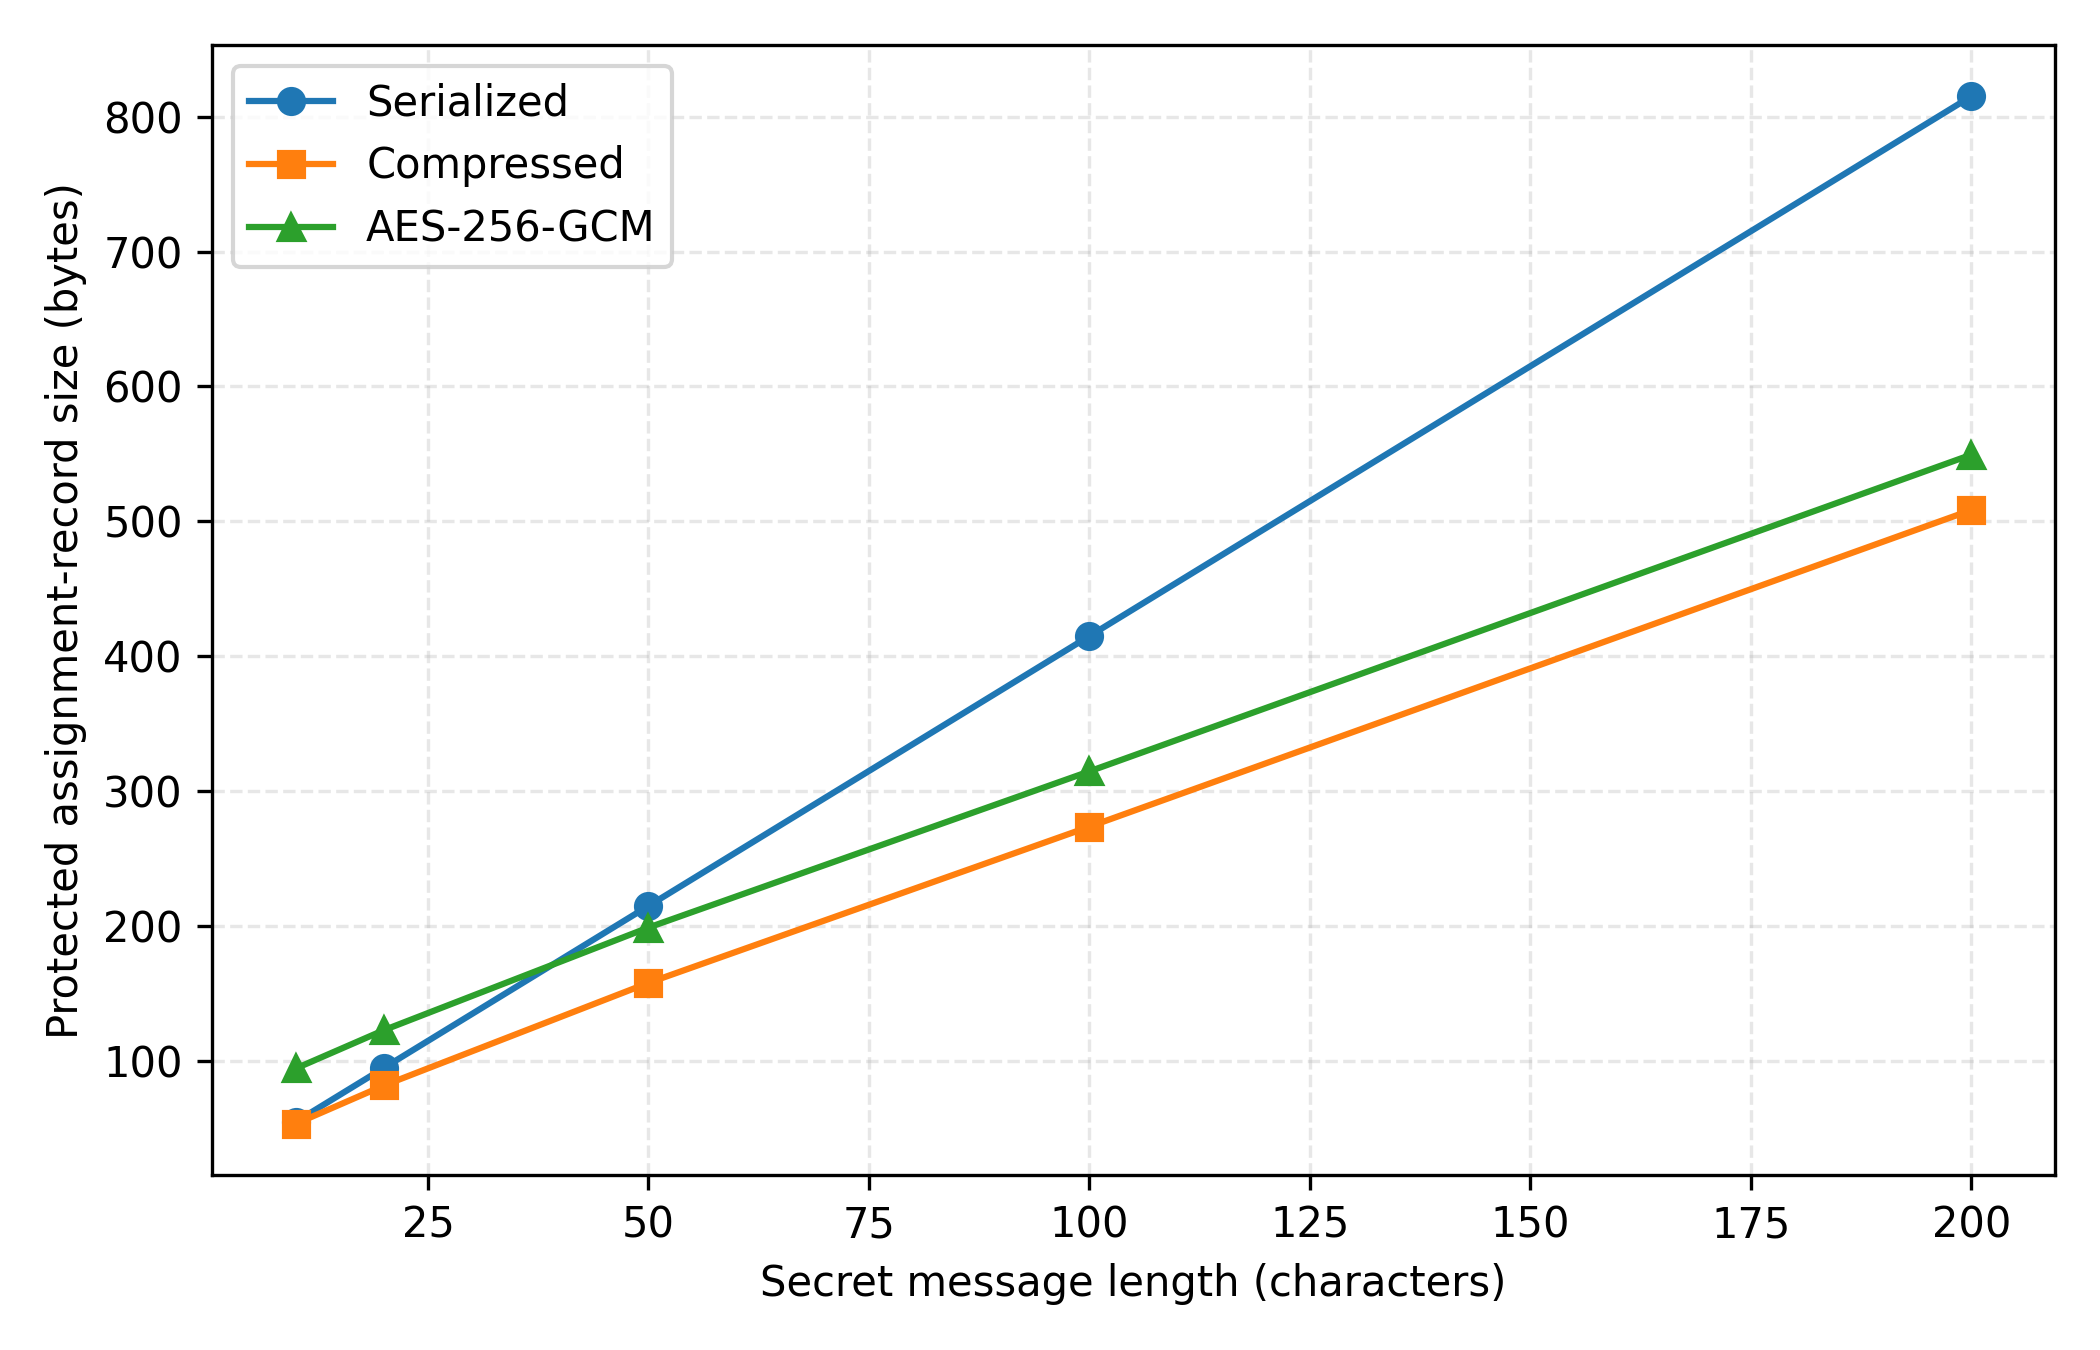
\includegraphics[width=\linewidth]{fig_auxiliary_channel.png}
\caption{Measured serialized, compressed, and AES-256-GCM assignment-record sizes.}
\label{fig:auxiliary_channel_real}
\end{figure}

For the compact representation, the encrypted-to-message byte ratio decreases
from 9.45 at 10 characters to 2.75 at 200 characters. Compact location tokens
reduce the 200-character envelope to 549.40 bytes, corresponding to 2.39 times
the directly encrypted message. The shaped 200-record envelope is constant at
852 bytes for all tested lengths, corresponding to 3.70 times the directly
encrypted 200-character message. This measurement makes the representation
cost explicit alongside FHAM's cover-conditioned assignment and unchanged
carrier. For a byte-level comparison, define the record payload fraction as
message bytes divided by transmitted record bytes, excluding the shared cover
and any transport framing. At 200 bytes this fraction is $200/549.40=36.4\%$
for the compact FHAM envelope and $200/852=23.5\%$ for the shaped envelope;
the directly protected-message baseline is $200/230.10=86.9\%$. These ratios
describe only the measured record representation and do not account for
cover-selection, synchronization, or network costs. AES-GCM detects
modification of the protected metadata before extraction. At 200 characters,
measured Python allocation peaks are
approximately 295 KiB for compact protection and 28 KiB for compact recovery;
the shaped mode avoids compression and uses fixed-capacity encrypted padding.

The length-sweep above uses the globally optimal unbounded assignment to
isolate serialization cost across message lengths. To quantify the same cost
under the principal bounded condition, we evaluated 200-character messages
with $B=2$ on the same controlled-image/message cohort
(eight images and ten messages per image). All 80 messages were feasible. The
Without pre-assignment source compression, the mean compact envelope was 549.88 bytes, compared with 230.10 bytes for direct
message protection, a ratio of 2.39 (Table~\ref{tab:channel_bounded}). The
bounded and unbounded records therefore have similar measured sizes in this
cohort. Direct encryption uses fewer bytes in this comparison; FHAM's measured
benefit concerns assignment feasibility under a fixed-cover representation,
not communication volume. Raw trial results are included with the
reproducibility files.

\begin{table}[!t]
\centering
\small
\caption{Compact record size for the controlled 200-character cohort under $B=2$, without pre-assignment source compression.}
\label{tab:channel_bounded}
\resizebox{\linewidth}{!}{%
\begin{tabular}{rrrrrr}
\toprule
\textbf{$B$} & \textbf{Feasible / 80} & \textbf{Raw record (B)} & \textbf{Compact envelope (B)} & \textbf{Direct encrypted (B)} & \textbf{Ratio} \\
\midrule
2 & 80 & 815.00 & 549.88 & 230.10 & 2.39 \\
\bottomrule
\end{tabular}
}

\end{table}

We also evaluated a packed-record coding prototype for the compressed
messages under the spectral $12\times12$, $B=2$ profile. It represents each
location token with 13 bits and each bounded residual with 3 bits, then applies
zlib and AES-256-GCM with the same nonce and authentication-tag lengths as the
compact format. The decoder reproduced every tested location--residual pair
and every source message exactly on the identity channel. Table
~\ref{tab:preprocessed_metadata} reports mean envelope sizes over eight
controlled images and three messages per family. For templated text, the
prototype reduces the compact FHAM envelope from 349.79 to 284.92 bytes; the
directly compressed and protected message is 145 bytes. For repeated-byte
messages, it reduces 97.92 to 87 bytes, while the direct encrypted baseline is
41 bytes. The packed representation therefore lowers record cost but does not
make FHAM smaller than direct encryption in these matched trials.

\begin{table}[!t]
\centering
\small
\caption{Protected Metadata after Lossless Message Compression (Bytes)}
\label{tab:preprocessed_metadata}
\resizebox{\linewidth}{!}{\begin{tabular}{lrrrrr}
\toprule
\textbf{Message family} & \textbf{Coded bytes} & \textbf{Compact FHAM} & \textbf{Packed FHAM prototype} & \textbf{Direct AES-GCM} & \textbf{Packed/direct} \\
\midrule
Repeated byte & 12 & 97.92 & 87.00 & 41.00 & 2.12 \\
Templated text & 116 & 349.79 & 284.92 & 145.00 & 1.96 \\
Printable ASCII & 201 & 535.92 & 422.88 & 230.00 & 1.84 \\
Uniform bytes & 211 & 557.08 & 438.17 & 240.00 & 1.83 \\
\bottomrule
\end{tabular}
}
\end{table}

The volume comparison uses an equally compressed plaintext for the direct
AES-GCM baseline. Under the compact format, envelope length remains observable
and tracks the compressed assignment length. Under the existing 200-record
shaped format, the envelope remains 852 bytes irrespective of the number of
compressed symbols. Thus source compression improves feasibility for
low-entropy messages and lowers compact-record size, while fixed-size shaping
retains a larger, length-independent record cost. Neither parameter tuning nor
the packed-record prototype reverses the measured direct-encryption volume
advantage.

\subsection{Message-Length Leakage Through Envelope Size}

AES-GCM guarantees confidentiality and integrity of the envelope contents,
but neither AES-GCM nor any generic authenticated encryption scheme hides
the length of its own ciphertext; treating ciphertext indistinguishability as
covering length observability would overstate the guarantee. We therefore
measure, rather than assume, how much an observer of the envelope size alone
can infer about message length. Table~\ref{tab:leakage} reports, over the
eight controlled images at five lengths (10-200 bytes, 400 trials per mode),
the Pearson correlation and the mutual information between message length and
the observed envelope size, both raw and after padding to the nearest
64-byte class. For the compact representation, the raw envelope size is almost
perfectly informative of length (Pearson $r=0.999$; mutual information
2.32 bits, matching $\log_2 5$ for the five tested lengths). Padding compact
envelopes to 64-byte classes collapses 92 distinct raw sizes into 6 classes
but still leaks 1.92 of the 2.32 maximum bits ($r=0.991$). The shaped
representation instead yields one observable size and one size class across
all tested lengths, reducing this measured size-only leakage to 0.00 bits.
This measurement quantifies the size-leakage reduction from replacing
variable compression and length-dependent records with a fixed-capacity
encrypted envelope.

\begin{table}[!t]
\centering
\caption{Message-Length Leakage Through Envelope Size (64-Byte Padding Classes)}
\label{tab:leakage}
{\small\setlength{\tabcolsep}{4pt}\begin{tabular}{lrrrrr}
\toprule
\textbf{Mode} & \textbf{Raw sizes} & \textbf{Size classes} & \textbf{$r$(length,size)} & \textbf{MI raw} & \textbf{MI class} \\
\midrule
Compact & 92 & 6 & 0.999 & 2.32 bits & 1.92 bits \\
Shaped & 1 & 1 & 0.000 & 0.00 bits & 0.00 bits \\
\bottomrule
\end{tabular}
}
\end{table}

\subsection{Traffic Detectability of the Protected Envelope}

AES-GCM protects envelope contents under its key and nonce assumptions;
envelope detectability is evaluated separately. We use an H0/H1 classifier
protocol in which H1 contains genuine FHAM records and H0 contains decoy
records matched by image, message length, record count, and residual bound.
Decoy locations are sampled from the same codebook, with residuals drawn
uniformly inside the bound. The two classes therefore differ in assignment
content. Four classifiers (logistic regression, random forest, gradient
boosting, and a small MLP) use final-size features and a local protection-time
proxy over 1,920 traces per envelope mode (8 images $\times$ 3 lengths
$\times$ 40 trials $\times$ 2 classes), with a stratified 70/30 train/test
split (Table~\ref{tab:traffic_detectability}). For compact envelopes, all
classifiers reach $\mathrm{AUC}=1.00$ against the 0.50 baseline: zlib
compresses the clustered, near-zero residuals of genuine global assignments
more effectively than uniformly random decoy residuals, creating a size
signal. For shaped envelopes, all classifiers reach $\mathrm{AUC}=0.50$ at
the fixed 852-byte record size under these features. The measurement covers
envelope size and the local protection-time proxy; packet timing, routing,
batching, and platform effects remain outside its feature set.

\begin{table}[!t]
\centering
\caption{H0/H1 Traffic Detectability by Envelope Mode (1920 Traces per Mode, 70/30 Train/Test Split)}
\label{tab:traffic_detectability}
{\small\setlength{\tabcolsep}{4pt}\begin{tabular}{llrrr}
\toprule
\textbf{Mode} & \textbf{Classifier} & \textbf{AUC} & \textbf{Bal. Acc.} & \textbf{TPR@5\%FPR} \\
\midrule
Compact & Logistic regression & 1.00 & 1.00 & 1.00 \\
Compact & Random forest & 1.00 & 1.00 & 1.00 \\
Compact & Gradient boosting & 1.00 & 1.00 & 1.00 \\
Compact & MLP & 1.00 & 1.00 & 1.00 \\
Compact & Random baseline & 0.50 & 0.50 & 0.05 \\
Shaped & Logistic regression & 0.50 & 0.50 & 0.00 \\
Shaped & Random forest & 0.50 & 0.50 & 0.00 \\
Shaped & Gradient boosting & 0.50 & 0.50 & 0.00 \\
Shaped & MLP & 0.50 & 0.50 & 0.00 \\
Shaped & Random baseline & 0.50 & 0.50 & 0.05 \\
\bottomrule
\end{tabular}
}
\end{table}

\subsection{Packet-Level Signature Baseline in Non-VPN Captures}

We additionally scanned the full-packet non-VPN portion of the ISCXVPN2016
dataset \cite{drapergil2016iscx,unbiscx2016}. The three downloaded archives
contain 109 PCAP/PCAPNG files with 21,919,108 packets. The dataset provides
labeled application sessions; its documentation states that unrelated
applications were closed during each targeted capture. It therefore provides
a labeled non-VPN baseline rather than mixed background traffic. We searched
decoded TCP and UDP packet payloads for the protocol markers used by the
implementation. The four-byte markers appeared 45 times across 9 captures:
30 \texttt{FHMS}, 8 \texttt{FHME}, and 7 \texttt{FHMT} packet-marker hits
(Table~\ref{tab:nonvpn_signature_baseline}). None of the 30 packet-local
\texttt{FHMS} matches was followed by the current protocol version byte
\texttt{01}; no packet-local \texttt{FHMS\,01} candidate was observed. The raw
four-byte magic is therefore not unique in this corpus, while the added version
byte removed the observed packet-local candidates.

This packet-local scan is a background signature baseline, not a detector
evaluation. We therefore performed a separate TCP-stream scan and generated
controlled positive traces for two explicitly defined transport profiles, as
described next. The positive traces are synthetic, and the background set is
not mixed traffic; these experiments consequently provide neither an
operational false-positive rate nor evidence of indistinguishability in
deployed network traffic.

\begin{table}[H]
\centering
\small
\caption{Packet-Local FHAM Marker Scan in the ISCXVPN2016 Non-VPN Captures}
\label{tab:nonvpn_signature_baseline}
\begin{tabular}{lr}
\toprule
Metric & Observed value \\
\midrule
Non-VPN capture files & 109 \\
Packets parsed & 21,919,108 \\
Payload packets containing \texttt{FHMS} & 30 \\
Payload packets containing \texttt{FHME} & 8 \\
Payload packets containing \texttt{FHMT} & 7 \\
Files containing at least one marker & 9/109 \\
Packet-local \texttt{FHMS\,01} matches & 0 \\
\bottomrule
\end{tabular}

\end{table}

\subsection{Synthetic FHAM Transport Pilot}

We generated controlled positive TCP captures to examine the observability of
the application framing under two transport profiles. The raw profile carries
the experimental FHAM frame directly over TCP. The second profile carries the
same application exchange in a locally generated TLS~1.3 session; the synthetic
client validates the locally pinned test certificate. Each exchange uses the
authenticated session and cover-binding implementation evaluated below. We
generated 40 flows for each of two message lengths (40 and 200 characters) and
each profile, across the eight controlled covers. The application-level
verification recovered every message and validated the key agreement and
cover binding in all 80 trials per profile. These are controlled software
captures, not captures from a deployed network service.

In the reconstructed TCP streams, all 80 raw-profile flows contained the
versioned \texttt{FHAM} frame marker, whereas none of the TLS~1.3 flows exposed
that application marker in the TCP payload. Across the 5,398 background TCP
flows reassembled from the 109 non-VPN captures, four contained the raw
four-byte substring \texttt{FHAM}; all four were in \texttt{scp1.pcapng}, and
none was followed by the version byte in the tested frame signature. Three
other flows in that capture reached the reassembler's 1-MB pending-buffer cap
and triggered resynchronization. Thus, the versioned-marker result applies to
the successfully reassembled stream regions; it is not an exhaustive claim
about bytes discarded during cap-triggered resynchronization.

The median flow sizes and packet counts for both synthetic profiles fell
individually within the central 10th--90th percentile interval of the
background distributions. This is a marginal range comparison: it does not
combine features into a classifier and does not establish that the positive
flows are statistically indistinguishable from ordinary traffic. In
particular, the ISCXVPN2016 captures are labeled application sessions recorded
with unrelated applications closed, rather than mixed background traffic.
This capture-feature comparison does not assess live TLS fingerprints,
application behavior, or selection effects from message-conditioned cover
choice. Relay timing and chunk features are evaluated in the matched
socket-level pilot below. Table~\ref{tab:transport_pilot} summarizes the
synthetic profile and background flow ranges.

\begin{table}[H]
\centering
\small
\caption{Synthetic positive-flow transport pilot and marginal comparison with reassembled non-VPN TCP flows.}
\label{tab:transport_pilot}
\begin{tabular}{llrrrrr}
\toprule
Transport & Length & Flows & Exact & Marker & Median & Median IP \\
profile & (chars) & & recovery & visible & packets & bytes \\
\midrule
Raw TCP & 40  & 40 & 40/40 & 40/40 & 8  & 837  \\
Raw TCP & 200 & 40 & 40/40 & 40/40 & 8  & 1,477 \\
TLS~1.3/TCP & 40  & 40 & 40/40 & 0/40 & 13 & 3,261 \\
TLS~1.3/TCP & 200 & 40 & 40/40 & 0/40 & 13 & 3,901 \\
\bottomrule
\end{tabular}

\vspace{2pt}
\parbox{\linewidth}{\footnotesize The marker column reports detection of the
versioned application-frame signature in reassembled TCP payloads. Median TCP
payload bytes were 517, 1,157, 2,741, and 3,381, respectively. For each row,
100\% of flows fell individually within the background central 10th--90th
percentile ranges for both packet count and IP-byte size; these marginal
comparisons are not a joint classifier.}

\end{table}

\subsection{Socket-Level FHAM Detectability Pilot}

We compared FHAM exchanges with ordinary HTTP/1.1 JSON request--response
controls over real local TCP sockets. For every FHAM exchange, the control
request and response had exactly the same respective plaintext byte lengths.
Both profiles used the same local client, relay, and server implementations;
the encrypted profile used the same TLS~1.3/OpenSSL configuration and pinned
certificate.
A transparent TCP relay observed the byte streams and their arrival times
without terminating TLS or saving payloads. Each profile comprised 80 matched
pairs per run, with three independently executed runs (240 pairs and 480
flows per profile). A logistic-regression detector was trained on two runs
and evaluated on the held-out third run, repeating this split for all runs.

On raw TCP, the versioned FHAM marker appeared in all 240 FHAM streams and in
none of the 240 HTTP controls. Under TLS~1.3, it appeared in neither class;
all 240 FHAM/control pairs had identical directional TLS record-length
sequences and directional wire-byte totals. The size-and-record detector
therefore had AUC 0.50 for both profiles. The held-out AUCs using relay
read-chunk and timing features were 0.461, 0.498, and 0.481 for raw TCP, and
0.514, 0.536, and 0.514 for TLS~1.3 (Table~\ref{tab:matched_tls_control}).
Every paired-bootstrap 95\% interval for these held-out timing-feature AUCs
included 0.50, so the detector did not show stable above-chance separation in
this matched local test.

The variable-length request remains visible in total volume: the FHAM client
sent 368 bytes at 40 characters and 1,008 bytes at 200 characters over raw
TCP, and 720 versus 1,360 TLS bytes under TLS~1.3. The corresponding HTTP
controls matched these totals by construction. This experiment establishes
marker visibility for the raw profile and tests content-versus-size leakage
with actual local TCP sockets. The matched controls isolate the effect of
application identity when directional volumes and TLS record lengths coincide;
the following experiment evaluates the same FHAM transport profile against
unmatched application flows.

\begin{table}[H]
\centering
\scriptsize
\setlength{\tabcolsep}{3pt}
\caption{Socket-level FHAM marker and held-out detectability results with matched HTTP controls.}
\label{tab:matched_tls_control}
\begin{tabular}{lrrrrr}
\toprule
Profile & Marker & Bytes & TLS records & AUC & Held-out relay \\
 & FHAM/HTTP & matched & matched & size/record & AUC by run \\
\midrule
Raw TCP & 240/0 & 240/240 & --- & 0.500 & .461, .498, .481 \\
TLS~1.3/TCP & 0/0 & 240/240 & 240/240 & 0.500 & .514, .536, .514 \\
\bottomrule
\end{tabular}

\vspace{2pt}
\parbox{\linewidth}{\footnotesize Each profile includes 240 matched pairs
(80 per independent run). Equal byte pairs match client and server directions;
for TLS~1.3, TLS record-length sequences also match in both directions. The
classifier trained on two runs and tested on the third. Each timing-feature
test used 80 held-out pairs; all paired-bootstrap 95\% intervals included
0.50.}

\end{table}

\subsection{Detectability Against Captured NonVPN TLS Traffic}

We next compared the 240 FHAM TLS~1.3/TCP flows with TLS flows reassembled from
109 PCAP/PCAPNG files in the ISCXVPN2016 NonVPN archives. The parser retained
1,946 flows across 91 captures containing at least three coherent TLS records
across both directions; the other 18 captures supplied no retained TLS flow.
The background includes application-oriented email, messaging, file-transfer,
streaming, and VoIP captures. A logistic-regression detector used only
directional TLS record counts, byte totals, and record lengths; TLS version,
addresses, ports, packet timing, and payload contents were excluded. Each fold
held out one complete FHAM socket run and one third of the background captures as
complete groups, training on the other two FHAM runs and the remaining
captures.

The held-out AUC was 0.957, 0.986, and 0.985 across the three runs, with
balanced accuracy of 0.923, 0.957, and 0.960 (Table~\ref{tab:nonvpn_tls_detectability}).
Byte totals alone gave AUCs of 0.650--0.739, and record counts alone gave
0.768--0.857; their combination gave 0.830--0.892. The first four record
lengths per direction gave 0.883--0.921; combining counts, byte totals, and
the first sixteen record lengths gave 0.957--0.986. Thus, the evaluated FHAM transport exchange is distinguishable
from these unmatched captured TLS flows through its observable size and record
sequence pattern. This is consistent with the matched-control experiment:
matching directional volumes and TLS record sequences removes that separation
for the paired HTTP exchanges.

These measurements establish a concrete traffic-detectability risk for the
tested application framing, server response, and TLS endpoint profile. The
positive flows use a local TLS endpoint, while the negative flows are
application-oriented captures from 2016; the experiment therefore evaluates
the complete measured profile against this corpus. A deployment profile can
reduce this signal by matching the joint request, response, record-length, and
timing distributions of its host application's ordinary traffic. The present
test provides a quantitative baseline for evaluating such traffic shaping;
it does not claim generalization to every contemporary network environment.

\begin{table}[H]
\centering
\scriptsize
\setlength{\tabcolsep}{3pt}
\caption{Held-out detection of FHAM TLS flows against captured NonVPN TLS traffic.}
\label{tab:nonvpn_tls_detectability}
\resizebox{\linewidth}{!}{%
\begin{tabular}{lrrrrrrrr}
\toprule
Run & Captures/flows & Bytes & Counts & Bytes+counts & First record & First 4 & Counts+bytes+16 & Bal. acc. \\
\midrule
rep1 & 31/702 & 0.650 & 0.774 & 0.830 & 0.648 & 0.883 & 0.957 & 0.923 \\
rep2 & 30/570 & 0.739 & 0.768 & 0.881 & 0.679 & 0.905 & 0.986 & 0.957 \\
rep3 & 30/674 & 0.714 & 0.857 & 0.892 & 0.601 & 0.921 & 0.985 & 0.960 \\
Mean & 30.3/649 & 0.701 & 0.799 & 0.868 & 0.643 & 0.903 & 0.976 & 0.947 \\
\bottomrule
\end{tabular}%
}

\end{table}

\subsection{Empirical TLS Padding and Record Fragmentation}

We implemented a transport-shaping profile using Windows Schannel TLS~1.2
session resumption. For each FHAM exchange, a framed padding record was
appended after the original offer and protected-record frames. The resulting
application byte stream was fragmented into TLS writes using a record profile
sampled from an independent subset of the NonVPN captures. The padding and
fragmentation were sized to match the sampled flow's directional TLS byte
totals and record counts exactly. An HTTP/1.1 JSON control was generated with
the same request and response lengths and write boundaries. The 240 FHAM
messages were verified by the assignment/envelope checks before transport;
the parser confirmed that the padding frame left the original serialized FHAM
frames intact.

We reserved 31 capture groups for shaping templates and used the other 60
groups (1,244 TLS flows) for held-out evaluation. Each of three independent
runs contained 80 FHAM/control pairs. Within each fold, one FHAM run and 20
complete evaluation captures were held out. The baseline and shaped profiles
were evaluated on the same capture groups with the same classifier.

The mean AUC for directional byte totals fell from 0.888 to 0.747, and the
record-count AUC fell from 0.909 to 0.594. Combining these features, AUC fell
from 0.929 to 0.781 (Table~\ref{tab:schannel_tls_padding}). The combined
counts, byte totals, and first-16-record profile changed from 0.974 to 0.955; the first-four
record detector measured 0.904 before shaping and 0.923 after shaping. This
profile therefore reduces the measured byte/count signal while the observed
early-record sequence remains discriminative. The result motivates shaping
connection setup together with application framing in subsequent protocol
work.

\begin{table}[H]
\centering
\scriptsize
\setlength{\tabcolsep}{3pt}
\caption{Mean held-out AUC for Schannel TLS~1.2 profiles against the same 60-capture evaluation set.}
\label{tab:schannel_tls_padding}
\begin{tabular}{lrrrrrr}
\toprule
Profile & Bytes & Counts & Bytes+counts & First record & First 4 & Counts+bytes+16 \\
\midrule
Unshaped & 0.888 & 0.909 & 0.929 & 0.686 & 0.904 & 0.974 \\
Padded and fragmented & 0.747 & 0.594 & 0.781 & 0.686 & 0.923 & 0.955 \\
\bottomrule
\end{tabular}

\end{table}

\subsection{Authenticated Session and Cover-Binding Pilot}

To evaluate the missing record-level protections, we implemented a session
profile with ephemeral X25519 key agreement, Ed25519 signatures over the
peer-bound key offers, and HKDF derivation of the AES-GCM session key
\cite{rfc7748,rfc8032,rfc5869,nist80038d}. The receiver authenticates each
offer against a provisioned identity public key. Each fixed-capacity record
authenticates the canonical reference-image digest, session identifier, and
sequence number as associated data. A persistent SQLite guard records the
next accepted sequence number and rejects records from unregistered sessions,
duplicate sequence numbers, and out-of-order records.

We evaluated eight controlled covers and five 40-character messages per
cover at $B=2$, using one session per cover. Across 40 records, session-key
agreement, exact message recovery, rejection of a one-pixel cover substitution,
rejection of a replay after reopening the replay-state database, and rejection
of an altered signed key offer each succeeded in 40/40 trials
(Table~\ref{tab:secure_channel_pilot}). A fixed 40-record capacity produced
236 bytes per protected record. The two signed ephemeral offers and the
session identifier add 208 bytes once per five-record session, or 277.60
bytes per message when amortized over this pilot's five records. This profile
therefore provides tested cover binding and persistent replay protection under
authenticated identity-key provisioning, while retaining a substantial
record-size cost. The pilot does not evaluate identity-key compromise; the
separate NonVPN TLS comparison quantifies detectability for this measured
endpoint profile and captured corpus.

\begin{table}[!t]
\centering
\small
\caption{Authenticated session, cover binding, persistent replay rejection, and communication overhead.}
\label{tab:secure_channel_pilot}
\begin{tabular}{lr}
\toprule
\textbf{Protocol check} & \textbf{Successful trials} \\
\midrule
X25519 session-key agreement & 40/40 \\
Exact message recovery & 40/40 \\
Wrong-cover envelope rejection & 40/40 \\
Persistent replay rejection & 40/40 \\
Altered key-offer rejection & 40/40 \\
Fixed record size ($r=40$) & 236 bytes \\
Signed session setup (amortized over 5 records) & 208 bytes/session \\
Record plus amortized setup per message & 277.60 bytes \\
\bottomrule
\end{tabular}

\end{table}

\subsection{Transformation Stress Test}

Table~\ref{tab:robustness} reports extraction with
the same metadata after applying transformations to the cover. The identity
case recovers every message. Under the evaluated transformations,
100-character recovery accuracy ranges from 8.2\% after a
$1^\circ$ rotation to 67.8\% after downscaling and restoration. These results
quantify the sensitivity of the evaluated spectral hash and define a concrete
target for integration with a transformation-stable descriptor.

\begin{table}[!t]
\centering
\caption{Recovery After Cover Transformations}
\label{tab:robustness}
\begin{tabular}{lrr}
\toprule
\textbf{Transformation} & \textbf{Exact (\%)} & \textbf{Characters (\%)} \\
\midrule
Identity & 100 & 100.0 \\
JPEG quality 90 & 0 & 62.9 \\
JPEG quality 75 & 0 & 46.0 \\
Resize 0.9 & 0 & 67.8 \\
Gaussian noise $\sigma=1$ & 0 & 59.4 \\
Gaussian noise $\sigma=2$ & 0 & 46.3 \\
Rotation $1^\circ$ & 0 & 8.2 \\
\bottomrule
\end{tabular}

\end{table}

Table~\ref{tab:comparative_robustness} compares three methods on 11 common
50-character cases. The cohort covers three controlled images, with five
deterministic messages per cover. Attacks follow the families reported by
WYSAWIS. These common-cohort reimplementation results use the datasets and
workflow specified in this study.

\begin{table*}[!t]
\centering
\caption{Common-Cohort Bit Accuracy for the Three Mapping Methods}
\label{tab:comparative_robustness}
\resizebox{\linewidth}{!}{\begin{tabular}{lrrr}
\toprule
\textbf{Attack} & \textbf{FHAM ($B=2$)} & \textbf{Abdulsattar Arr.4} & \textbf{WYSAWIS core} \\
\midrule
Identity & 100.0\% & 100.0\% & 100.0\% \\
Speckle noise, $v=0.005$ & 71.2\% & 61.7\% & 57.5\% \\
Salt-and-pepper, $v=0.005$ & 80.7\% & 86.4\% & 97.3\% \\
Gaussian filter, $5\times5$ & 84.0\% & 81.2\% & 31.3\% \\
Median filter, $5\times5$ & 76.4\% & 77.6\% & 37.4\% \\
\bottomrule
\end{tabular}
}
\end{table*}

WYSAWIS is strongest under the tested sparse salt-and-pepper corruption, with
72.7\% exact message recovery. All methods recover identity cases exactly.
FHAM retains the most bits
under speckle and Gaussian filtering, while Abdulsattar is marginally higher
under median filtering. The attack-dependent ordering highlights complementary
feature behavior and motivates a broader robustness benchmark.

\subsection{Extended Transformation Matrix}

Table~\ref{tab:robustness} covers 7 conditions. To characterize the spectral
descriptor's transformation sensitivity more completely, we additionally
evaluate a 36-condition matrix plus the identity reference, produced by
\texttt{extended\_transformation\_robustness\_experiment}, spanning 5 JPEG
qualities, 4 resize-and-restore ratios, 4 rotation angles, 3 Gaussian-noise
levels, 2 speckle levels, 2 impulse-noise densities, 2 Gaussian-filter and 2
median-filter kernels, 6 photometric changes (brightness, contrast, gamma),
2 crop-and-restore levels, and 4 combined transforms, over the eight
controlled images at 100 bytes (40 trials per condition). Table~\ref{tab:extended_robustness}
reports the range of mean character accuracy within each category; the full
36-row table is in \texttt{results/extended\_robustness.csv}. No non-identity
condition reaches exact message recovery, consistent with
Table~\ref{tab:robustness}. Cropping is the most destructive category tested
(0.35\% character accuracy at 5\% crop, 6.8\% at 1\%), because it shifts
every block position relative to the assignment's stored coordinates.
Rotation is comparably severe (8.2--19.8\%) for the same reason at a smaller
spatial scale. Photometric changes are the mildest category (76.7--97.2\%),
since brightness, contrast, and gamma adjustments preserve the ordinal
comparisons the spectral hash relies on more often than geometric changes
do. JPEG compression, resizing, noise, and filtering fall between these
extremes and degrade gradually with severity (e.g., 68.1\% at JPEG quality 95
down to 34.9\% at quality 50). This extended matrix broadens the
transformation coverage and confirms the conclusion from Table~\ref{tab:robustness}:
the evaluated spectral descriptor has limited robustness to geometric transformations.

\begin{table}[!t]
\centering
\caption{Extended Transformation Matrix: Character Accuracy Range by Category (100 Bytes, 40 Trials per Condition)}
\label{tab:extended_robustness}
\begin{tabular}{lrr}
\toprule
\textbf{Category (conditions)} & \textbf{Min (\%)} & \textbf{Max (\%)} \\
\midrule
JPEG quality (5) & 34.9 & 68.0 \\
Resize-restore (4) & 62.4 & 81.4 \\
Rotation (4) & 8.2 & 19.8 \\
Gaussian noise (3) & 45.4 & 68.2 \\
Speckle noise (2) & 22.5 & 34.9 \\
Impulse noise (2) & 27.8 & 73.2 \\
Gaussian/median filter (4) & 27.0 & 56.0 \\
Photometric (6) & 76.6 & 97.2 \\
Crop-restore (2) & 0.4 & 6.8 \\
Combined (4) & 53.6 & 58.1 \\
Identity (1) & \multicolumn{2}{c}{100.0} \\
\bottomrule
\end{tabular}

\end{table}

\subsection{External Corpus Validation}

To move beyond the manifest-integrity smoke test, Table~\ref{tab:external_corpus}
evaluates FHAM ($B=2$, spectral descriptor) on 60 images independently drawn
from each of BOSSBase~1.01, BOWS2, and COCO~2017 validation (180 images total,
none shared with the controlled or stress corpora), using deterministic messages from the same manifest as Table~\ref{tab:message_family} at 50 and 100
bytes. The benchmark message quota includes five 50-byte messages and one
100-byte message per family for each of 60 images (300 and 60 trials per
dataset-family cell). The 100-byte external proportions provide corroborative
evidence, with fewer trials than the 50-byte condition. Results closely track
the controlled-corpus pattern: printable ASCII and uniform bytes remain fully
feasible at both lengths on all three external datasets, templated natural-language text stays
at or above 95\% at 100 bytes, and the adversarial repeated-byte family
collapses to 0\% at 100 bytes on every external dataset, consistent with the
multiplicity-saturation mechanism identified on the controlled corpus. This is
a bounded check at two message lengths and 60 images per corpus, focused on
message-family coverage; the transformation channel is checked separately at
the larger, approximately 2000-image-per-corpus scale in
Table~\ref{tab:stratified_robustness}. The three-corpus message-family check
uses 50- and 100-byte messages, while 200-byte assignment evidence is available
for the controlled and stress corpora and the disjoint 100-image BOSSBase
descriptor-validation sample. Accordingly, cross-dataset generalization at
200 bytes is characterized by the BOSSBase sample; the larger three-corpus
robustness study uses 100-byte messages.

\begin{table*}[!t]
\centering
\caption{External-Corpus Assignment Feasibility by Dataset and Message Family (60 Images per Dataset)}
\label{tab:external_corpus}
\resizebox{\linewidth}{!}{\begin{tabular}{lrrrrrr}
\toprule
& \multicolumn{3}{c}{\shortstack{\textbf{50 bytes}\\\textbf{(300 trials)}}} & \multicolumn{3}{c}{\shortstack{\textbf{100 bytes}\\\textbf{(60 trials)}}} \\
\textbf{Family} & \textbf{BOSSBase} & \textbf{BOWS2} & \textbf{COCO2017} & \textbf{BOSSBase} & \textbf{BOWS2} & \textbf{COCO2017} \\
\midrule
Adversarial repeated & 84.7\% & 90.3\% & 90.7\% & 0.0\% & 0.0\% & 0.0\% \\
Natural text & 100.0\% & 100.0\% & 100.0\% & 100.0\% & 98.3\% & 95.0\% \\
Printable ASCII & 100.0\% & 100.0\% & 100.0\% & 100.0\% & 100.0\% & 100.0\% \\
Uniform bytes & 100.0\% & 100.0\% & 100.0\% & 100.0\% & 100.0\% & 100.0\% \\
\bottomrule
\end{tabular}
}
\end{table*}

\subsection{Stratified Robustness Check at Corpus Scale}

The external check above uses 60 images per corpus. To validate the
transformation-sensitivity findings of Table~\ref{tab:extended_robustness} at
a scale closer to the full corpora, Table~\ref{tab:stratified_robustness}
repeats a
moderate 8-condition channel (identity, JPEG quality 90/75, resize 0.90,
$1^\circ$ rotation, Gaussian noise $\sigma=1$, and $3\times3$ Gaussian/median
filtering) on a deterministic, evenly spaced stratified sample of
approximately 2000 images from each of BOSSBase~1.01, BOWS2, and COCO~2017
validation (1998, 1998, and 1999 images respectively; one 100-byte message
per image, $B=2$). The pattern already observed on the controlled corpus and
on the 180-image external sample holds at this larger scale: identity
recovers every message exactly on all three corpora; rotation by $1^\circ$
remains the most damaging condition (7.3--7.8\% character accuracy); the
remaining conditions degrade gradually (43--81\%) and never reach exact
recovery. No dataset shows qualitatively different behavior from the other
two, indicating that the spectral descriptor's transformation sensitivity is
a property of the descriptor rather than an artifact of the controlled
corpus.

\begin{table}[!t]
\centering
\caption{Stratified Robustness Check (100 Bytes, $\approx$2000 Images per Corpus)}
\label{tab:stratified_robustness}
\begin{tabular}{lrrr}
\toprule
\textbf{Transform} & \textbf{BOSSBase} & \textbf{BOWS2} & \textbf{COCO2017} \\
\midrule
Identity & 100.0\% & 100.0\% & 100.0\% \\
JPEG quality 90 & 61.0\% & 63.3\% & 69.7\% \\
JPEG quality 75 & 46.4\% & 47.3\% & 55.9\% \\
Resize 0.90 & 66.3\% & 80.7\% & 71.7\% \\
Rotation $1^\circ$ & 7.5\% & 7.3\% & 7.8\% \\
Gaussian noise $\sigma{=}1$ & 58.5\% & 56.5\% & 71.0\% \\
Gaussian filter $3\times3$ & 54.5\% & 58.1\% & 56.0\% \\
Median filter $3\times3$ & 45.5\% & 58.3\% & 43.2\% \\
\bottomrule
\end{tabular}

\end{table}

\subsection{Message-Layer Error Correction}
\label{sec:ecc}

The transformation study above characterizes a per-symbol failure profile,
not an exact-recovery guarantee: even a substantial per-character accuracy
improvement cannot, by itself, raise the probability that all symbols of a
length-$L$ message survive simultaneously, since exact recovery requires
every symbol to be correct. Rather than pursue further descriptor-level
tuning, we test a message-layer repetition code: \texttt{fham.ecc} expands
each character into $r$ consecutive copies before assignment
(\texttt{repetition\_encode}) and reconstructs it by per-position majority
vote after extraction (\texttt{repetition\_decode}), at a capacity cost of
one usable character per $r$ locations consumed. This changes nothing in
the descriptor or the \texttt{Location} model; it only adds redundancy at
the message layer, the standard mechanism by which robust watermarking and
data-hiding literature accommodates a noisy channel instead of demanding a
noiseless one.

\texttt{ecc\_repetition\_experiment} repeats the extended transformation
matrix (Table~\ref{tab:extended_robustness}'s 36 conditions plus identity)
at $r \in \{1,3,5\}$ on 40-byte messages (20 trials per image), partitioning
conditions into a \emph{value} domain (JPEG, noise, filtering, resizing,
photometric change; 30 conditions) and a \emph{geometric} domain (rotation,
crop-restore; 6 conditions, listed in \texttt{GEOMETRIC\_TRANSFORMS}).
Table~\ref{tab:ecc_repetition} reports exact recovery and character accuracy
averaged within each domain. In the value domain, $r=5$ raises exact
recovery from 4.2\% to 30.4\% (a 7.2$\times$ improvement) and character
accuracy from 58.8\% to 82.2\%. In the geometric domain, exact recovery
remains 0.0\% at every repeat factor tested, although character accuracy
still rises (9.4\% to 21.5\%): a repetition code corrects a minority of
corrupted copies only when the underlying per-copy signal retains some
correlation with the original symbol, whereas under rotation and crop the
recomputed descriptor at a fixed stored location is decorrelated from its
embed-time value rather than merely noisy, so majority vote over
decorrelated copies converges on nothing in particular.

\begin{table*}[!t]
\centering
\caption{Repetition-Code Error Correction: Exact Recovery and Character Accuracy by Domain (40 Bytes, 20 Trials per Image)}
\label{tab:ecc_repetition}
{\scriptsize\setlength{\tabcolsep}{2pt}\begin{tabular}{rrrrr}
\toprule
\textbf{Repeat} & \textbf{Value exact} & \textbf{Value char. acc.} & \textbf{Geom. exact} & \textbf{Geom. char. acc.} \\
\midrule
1 & 4.2\% & 58.8\% & 0.0\% & 9.4\% \\
3 & 9.3\% & 70.7\% & 0.0\% & 16.0\% \\
5 & 30.4\% & 82.2\% & 0.0\% & 21.5\% \\
\bottomrule
\end{tabular}
}
\end{table*}

This repetition-code experiment addresses value-domain corruption through a
capacity-costed mechanism. Repetition alone leaves fixed-coordinate geometric
errors unresolved because the stored locations still need correspondence to
the transformed image. A general detected-location assignment would replace
the fixed-coordinate \texttt{Location} representation and require
re-deriving Hall's feasibility characterization for the detected location
set. The following pilot evaluates ORB/RANSAC registration and a separate
closed-set route that retrieves the canonical reference and reuses its
original coordinates.

\subsection{Location Detection Errors and Synchronization}
\label{sec:detection_errors}

Let $\widehat{\mathcal{P}}$ be the set of locations detected after a cover
transformation, with hash values $\widehat{h}(p)$. Conditional on this
detected set, the bounded-assignment graph is formed by connecting message
position $j$ to detected location $p$ when
$|\alpha_j-\widehat{h}(p)|\leq B$. Hall's condition remains the exact
necessary-and-sufficient condition for a matching in this detected graph.
Missed detections remove right-side vertices and may remove feasible edges;
false detections add candidate vertices and edges. A matching in the detected
graph alone does not establish that a detected location corresponds to the
sender's location or that its recomputed hash preserves the transmitted
symbol. Exact recovery therefore requires both a feasible assignment and
correct sender--receiver location correspondence with sufficiently stable
hash values.

For a scale estimate, consider an idealized model in which each of $n$
message locations is independently detected and correctly matched with
probability $p$, with perfect correspondence precision and stable hash values.
The probability that every location required for exact recovery is matched is
$p^n$. Requiring an exact-recovery probability of at least $q$ gives
$p\geq q^{1/n}$. At a 95\% target, the resulting per-location thresholds are
99.872\% for $n=40$, 99.949\% for $n=100$, 99.974\% for $n=200$, and
99.987\% for $n=400$. These values quantify the all-symbol requirement under
independent detections, perfect correspondence precision, stable hash values,
and repetition factor $r=1$. A practical synchronization evaluation should report
location repeatability, correspondence precision, and downstream exact
recovery under specified transformations; detector performance can differ
when detections are dependent, correspondences are uncertain, hash values
change, or error correction is applied.

An exploratory registration and reference-retrieval pilot separates pixel
alignment from recovery through a shared canonical codebook. On each of the
eight controlled query covers, five 40-character messages were assigned with
$B=2$ and evaluated after a $1^\circ$ rotation and 5\% crop--restore
transformation. ORB keypoints and binary descriptors \cite{rublee2011orb}
were matched with cross-checking and a 0.8 ratio threshold. For cover
identification, each transformed query was matched against a closed gallery
of 219 canonical stress-corpus covers; candidates were ranked by descriptor
match count, and RANSAC inlier support selected among the ten highest-ranked
candidates. The eight query images were byte-identical to their canonical
gallery entries. Cover identity was recovered for all eight transformed
queries under each attack (8/8 per condition).

For the direct pixel path, RANSAC used random seed 20261110, at least four
matches, and a 3-pixel inlier threshold. Inverse-warping the transformed
pixels improved mean character accuracy from 6.88\% to 39.56\% under rotation
and from 0.25\% to 31.00\% under crop--restore, but exact recovery from those
registered pixels remained 0/40 for each condition. In the catalog path, the
receiver uses the identified cover's canonical copy and the original
location--residual record. This yielded exact recovery in 40/40 messages per
condition (Table~\ref{tab:geometry_registration_pilot}). The result shows
that cover-level synchronization to a known reference can restore exact
recovery in this closed-set pilot even when interpolated pixels perturb the
hashes. It does not establish open-set rejection, performance on near-duplicate
references, or retrieval over larger and independently sourced galleries.

\begin{table}[!t]
\centering
\small
\caption{Geometric pilot: closed-set cover identification in a 219-image gallery and message recovery over canonical references (40 messages per condition).}
\label{tab:geometry_registration_pilot}
\resizebox{\linewidth}{!}{%
\begin{tabular}{lrrrrr}
\toprule
\textbf{Transform} & \textbf{Gallery} & \textbf{Cover ID} & \textbf{Exact messages} & \textbf{Char. acc., fixed (\%)} & \textbf{Char. acc., warped (\%)} \\
\midrule
$1^\circ$ rotation & 219 & 8/8 & 40/40 & 6.88 & 39.56 \\
5\% crop--restore & 219 & 8/8 & 40/40 & 0.25 & 31.00 \\
\bottomrule
\end{tabular}
}

\end{table}

\subsection{Discussion and Scope}

The experiments characterize FHAM as a reusable fixed-cover assignment layer.
The descriptor supplies hash-indexed locations, FHAM computes bounded
injective assignments, and the protected-envelope evaluation measures the
associated record size and selected leakage. The session pilot adds key
agreement, cover binding, and durable replay handling to this record protocol.
Complete communication performance also depends on identity-key provisioning,
cover-selection policy, transport concealment, and reference-catalog
availability.

Abdulsattar is the closest structural baseline: it assigns ASCII symbols to
locations within one cover using exact hash equality. Its overlapping layout
provides 6,889 locations, while long-message feasibility remains constrained by
hash-value multiplicity. FHAM addresses that constraint through bounded,
global assignment and an authenticated external record. WYSAWIS represents
message segments through category/rank codes and a large shared cloud corpus.
The comparison therefore spans distinct capacity, cover-selection, and
metadata-cost designs. At the tested bound, FHAM accepts more as-given covers
than the exact-match baseline and incurs a larger per-symbol record cost.

Message-family results show that effective capacity depends jointly on
message-value multiplicity and cover statistics. Uniform-byte and printable
messages remain highly feasible at longer lengths, while repeated-byte content
causes feasibility to collapse in the controlled and external corpora. The
causal codebook ablation isolates the bounded/global assignment gain: under a
common descriptor protocol, changing the assignment rule yields 92.5--100\%
success across all four tested codebooks, including Abdulsattar's. The fixed
eligibility procedure selects the spectral descriptor on the disjoint
BOSSBase validation sample. Dense and aggregated formulations agree on
feasibility and optimal cost across the 160 feasible comparison trials; their
runtime and memory trade-offs are detailed in Table~\ref{tab:formulation_comparison}.

The compact protected envelope exposes message length through its raw size,
including after fixed-class padding. The shaped fixed-capacity record reduces
the measured size-only leakage to 0.00 bits at 852 bytes. The 36-condition
transformation matrix and stratified evaluation on about 2,000 images per
corpus show consistent geometric sensitivity across BOSSBase, BOWS2, and
COCO~2017, with rotation and cropping producing the largest degradation. The
stability-aware cost improves validation character accuracy over pure residual
minimization, while exact recovery remains 0\% under the tested validation
channel. Message-level repetition improves exact recovery for value-domain
transformations at proportional capacity cost. Direct extraction from
registered, transformed pixels remains at 0.0\% exact recovery, while the
closed-set reference-catalog pilot recovers all tested messages from their
canonical covers. In the envelope-detection experiment, compact records are
distinguishable from matched-shape decoys through compressed residual size,
while shaped records yield AUC 0.50 for the tested size and local timing-proxy
features. Together, these results define FHAM's assignment capacity,
robustness, metadata cost, and measured envelope-detection profile.

\section{Conclusion}
\label{sec:conclusion}

FHAM formalizes intra-cover hash mapping as a bounded injective assignment.
Hall's condition characterizes feasibility, and rectangular linear assignment
minimizes total residual cost. With $B=2$, assignment feasibility was 100\%
through length 200 on the eight controlled covers and 74.4\% at length 200 on
the 219-image stress corpus; these values describe assignment feasibility on
the original cover. Effective capacity also depends on message-value
distribution: at length 200 in the controlled message-family experiment,
feasibility was 100\% for uniform-byte and printable-ASCII messages, 12.5\%
for templated text, and 0\% for repeated-byte messages. The bounded assignment
addresses a precise fixed-cover multiplicity problem whose effective capacity
varies with message distribution.

The parameter ablation identifies lossless pre-assignment compression and
smaller spectral blocks as effective capacity controls. On 200 LFW covers,
zlib preprocessing with a $12\times12$ profile raises $B=2$ feasibility for
200-byte repeated messages from 0\% to 97.8\% and for templated text from
80.5\% to 92.2\%; the 11-image scene holdout reports 100\% for repeated-byte
messages and 97.0\% for templated text. Increasing the bound to $B=4$ raises the corresponding LFW rates
to 98.5\% and 97.2\%. This gain is conditional on message compressibility;
zlib expands the tested uniform-byte and printable-ASCII inputs slightly.
The smaller blocks also increase codebook-construction time, and these
assignment results do not imply successful recovery after channel distortion.

FHAM uses the preprocessed cover as a shared reference and carries the
location--residual reconstruction record externally; image pixels remain
unchanged across assignments. In the measured 200-symbol condition, the
unbounded compact protected record was 549.40 bytes, compared with 230.10 bytes
for the directly protected message baseline; the fixed-capacity shaped record
was 852 bytes. Under the bounded $B=2$ cohort, the compact record averaged
549.88 bytes for the same 230.10-byte direct baseline. These measurements
characterize record-size cost alongside direct encryption. Direct encryption
uses fewer bytes in these tests. FHAM contributes a formal feasibility and
minimum-cost assignment interface for architectures whose representation is
defined by a fixed, unchanged cover; the measured assignment gains are reported
with their record-size cost.
For compressed 200-byte messages under the spectral $12\times12$, $B=2$
profile, a packed-record prototype lowers the mean compact FHAM envelope to
87--439 bytes across the four message families; the directly compressed and
protected messages require 41--240 bytes. The packed encoding is an
experimental record representation and does not reverse the measured
communication-volume comparison. Compact envelopes expose coded length, while
the fixed-capacity shaped envelope remains 852 bytes for a 200-record class.
The session profile binds each record to the canonical cover and rejects
replayed sequence numbers under persistent receiver state. The packet-level
and reassembled-stream scans provide a non-VPN background baseline for visible
record markers. The synthetic transport pilot measures marker visibility and
marginal flow-size and packet-count ranges for raw TCP and TLS~1.3/TCP profiles.
The socket-level pilot adds 240 same-size HTTP control pairs per profile and
leave-one-run-out classification over actual local TCP streams. Raw-TCP marker
detection is exact in this controlled comparison; TLS~1.3 hides the marker,
and the size/record classifier yields AUC 0.50. Relay timing/chunk classifiers
remain near chance across held-out runs. Against captured NonVPN TLS traffic,
the detector combining directional record counts, byte totals, and the first
16 record lengths achieves mean AUC 0.976. Empirical padding and fragmentation
reduce the combined byte-total/record-count AUC from 0.929 to 0.781 on a
disjoint capture subset, while the detector using those features plus the
first 16 record lengths reaches 0.955. Contemporary
mixed-network generalization, connection-setup shaping, and message-conditioned
cover-selection effects remain for further evaluation.

The transformation experiments confirm that rotation and cropping disrupt
fixed-coordinate extraction from transformed pixels: exact recovery remains
0/40 after inverse warping in the pilot. A complementary closed-set method
identifies each transformed query among 219 canonical references (8/8 covers
per transformation) and recovers all 40 messages per condition using those
canonical images. This result establishes exact recovery when the receiver
maintains a catalog containing the sender's reference. Open-set rejection,
near-duplicate covers, and substantially larger independent catalogs remain
to be evaluated.

The authenticated session profile derives per-session AES-GCM keys from
ephemeral X25519 offers authenticated by Ed25519, binds the envelope to the
canonical image, and rejects replays using persistent sequence state. The
pilot assumes authenticated identity keys and durable replay storage. The
H0/H1 envelope test compares matched-shape decoys. The transport pilot adds
synthetic raw-TCP and TLS~1.3/TCP positive flows and reassembles the available
non-VPN TCP background. The socket-level pilot directly compares each FHAM
flow with a same-size HTTP control and evaluates a held-out-run classifier on
the observed TCP streams. It confirms marker visibility in raw TCP and shows
that size/record features alone do not separate same-size FHAM and HTTP
exchanges under TLS~1.3. A capture-group-held-out comparison against 1,946
NonVPN TLS flows yields mean AUC 0.976 for directional counts, byte totals,
and the first 16 record lengths. The Schannel padding pilot reduces the
combined byte-total/record-count AUC from 0.929 to 0.781 on 1,244 disjoint
evaluation flows; adding the first 16 record lengths yields AUC 0.955. These measurements characterize
the tested endpoints and capture corpus, and establish an empirical baseline
for connection-setup and application-profile shaping.

\section*{Acknowledgements}
The authors gratefully acknowledge the support of the Abdus Salam International Centre for Theoretical Physics (ICTP) through its Associates Programme.

\section*{Funding}
This research received no specific grant from any funding agency in the public, commercial, or not-for-profit sectors.
\section*{Declaration of Competing Interest}
The authors declare that they have no known competing financial interests or personal relationships that could have appeared to influence the work reported in this paper.
\section*{Ethics Statement}
Not applicable. The study performs secondary use of existing public research image datasets and involves no new data collection, participant recruitment, biometric identification, re-identification, or inference about depicted persons.
\section*{Data Availability}
Exact controlled/stress inputs used in the main experiments and their provenance manifests are supplied in Supplementary Material S2. BOSSBase~1.01, BOWS2, and COCO~2017 validation are third-party research datasets and are referenced through source instructions, relative filenames, preprocessing information, and SHA-256 manifests rather than redistributed. Supplementary Material S1 documents the dataset protocol and provenance interface.

\section*{Code Availability}
The implementation, automated test suite, experiment configuration, dataset/message manifests, analysis scripts, generated tables/figures, and raw/processed trial results supporting the reported claims are supplied as Supplementary Material S2. The corresponding public source snapshot is available at commit \href{https://github.com/EkodeckStephane/FHAM/tree/a7849bb}{a7849bb}.
\section*{Author Contributions}
Habibatou Mindja: Investigation, data curation, validation, writing--original draft, writing--review and editing. Ibrahima Tour\'e: Investigation, validation, writing--review and editing. St\'ephane Ga\"el R. Ekodeck: Conceptualization, methodology, formal analysis, software, validation, investigation, writing--original draft, writing--review and editing. Serge Alain Ebele: Conceptualization, methodology, formal analysis, writing--review and editing. Leonel Moyou Metcheka: Software, data curation, validation, writing--review and editing. Daniel Tieudjo: Software, data curation, validation, writing--review and editing, Supervision. Ren\'e Ndoundam: Conceptualization, Supervision, project administration, formal analysis, writing--review and editing.
\section*{Supplementary Material}
Supplementary Material S1 provides protocol and provenance details. Supplementary Material S2 contains the reproducibility artefact, including code, tests, manifests, and the results supporting the reported evidence. Third-party external-corpus images are obtained from their original distributors.
\section*{Declaration of generative AI and AI-assisted technologies in the manuscript preparation process}
During preparation of this manuscript, the authors used OpenAI ChatGPT (Codex) to support literature review, organize reviewer-driven revisions, and refine manuscript structure and language. The authors reviewed and edited the material and take full responsibility for the final content.
\begin{thebibliography}{28}

\bibitem{johnson1998exploring}
Johnson, N. F., \& Jajodia, S. (1998). Exploring steganography: Seeing the unseen. Computer, 31(2), 26–34. https://doi.org/10.1109/mc.1998.4655281

\bibitem{rublee2011orb}
Rublee, E., Rabaud, V., Konolige, K., \& Bradski, G. (2011). ORB: An efficient alternative to SIFT or SURF. In Proceedings of the 2011 IEEE International Conference on Computer Vision (pp. 2564--2571). https://doi.org/10.1109/ICCV.2011.6126544

\bibitem{chan2004hiding}
Chan, C.-K., \& Cheng, L.-M. (2004). Hiding data in images by simple LSB substitution. Pattern Recognition, 37(3), 469–474. https://doi.org/10.1016/j.patcog.2003.08.007

\bibitem{fridrich2012rich}
 Fridrich, J., \& Kodovský, J. (2012). Rich models for steganalysis of digital images. IEEE Transactions on Information Forensics and Security, 7(3), 868–882. https://doi.org/10.1109/TIFS.2012.2190402

\bibitem{xu2016structural}
Xu, G., Wu, H.-Z., \& Shi, Y.-Q. (2016). Structural design of convolutional neural networks for steganalysis. IEEE Signal Processing Letters, 23(5), 708–712. https://doi.org/10.1109/LSP.2016.2548421

\bibitem{zhou2015coverless}
Zhou, Z., Sun, H., Harit, R., Chen, X., \& Sun, X. (2015). Coverless image steganography without embedding. In Proceedings of ICCCS (pp. 123–132). https://doi.org/10.1007/978-3-319-27051-7\_11

\bibitem{zheng2018coverless}
Zheng, S., Wang, L., Ling, B., \& Hu, D. (2017). Coverless information hiding based on robust image hashing. In Proceedings of ICIC (pp. 536–547). https://doi.org/10.1007/978-3-319-63315-2\_47

\bibitem{wysawis2024} 
Fotso, D. B. M., Ebele, S. A., Ekodeck, S. G. R., \& Ndoundam, R. (2025). A high-capacity coverless image steganography approach using block-level hash encoding and sequence category mapping: WYSAWIS. Multimedia Tools and Applications, 84(42), 50173-50198. https://doi.org/10.1007/s11042-025-21128-y

\bibitem{abdulsattar2021}
Abdulsattar, F. S. (2021). Towards a high capacity coverless information hiding approach. Multimedia Tools and Applications, 80, 18821--18837. https://doi.org/10.1007/s11042-021-10608-6

\bibitem{qin2020gan}
Qin, J., Wang, J., Tan, Y., Huang, H., Xiang, X., \& He, Z. (2020). Coverless image steganography based on generative adversarial network. Mathematics, 8(9), 1394. https://doi.org/10.3390/math8091394

\bibitem{tan2024review}
Meng, L., Jiang, X., \& Sun, T. (2024). A review of coverless steganography. Neurocomputing, 566, 126945. https://doi.org/10.1016/j.neucom.2023.126945

\bibitem{li2024surf}
Li, F., Liu, C., Dong, Z., Sun, Z., \& Qian, W. (2024). A robust coverless image steganography algorithm based on image retrieval with SURF features. Security and Communication Networks, 2024, 5034640. https://doi.org/10.1155/2024/5034640

\bibitem{guo2024diverse}
Guo, B., Ping, P., \& Xu, F. (2025). Highly robust and diverse coverless image steganography against passive and active steganalysis. IEEE Transactions on Dependable and Secure Computing. https://doi.org/10.1109/TDSC.2024.3521424

\bibitem{ren2024joint}
Ren, C., \& Wu, B. (2024). A robust joint coverless image steganography scheme based on two independent modules. Cybersecurity, 7, 73. https://doi.org/10.1186/s42400-024-00299-5

\bibitem{guo2026capacity}
Guo, B., \& Ping, P. (2026). Towards robust and high-capacity coverless image steganography. Knowledge-Based Systems, 338, 115472. https://doi.org/10.1016/j.knosys.2026.115472


\bibitem{xiang2025survey}
Xiang, X., Tan, Y., Qin, J., \& Tan, Y. (2025). Advancements and challenges in coverless image steganography: A survey. Signal Processing, 228, 109761. https://doi.org/10.1016/j.sigpro.2024.109761

\bibitem{zhang2026diffusion}
Zhang, S., Xue, J., Fu, J., \& An, D. (2026). A review of generative coverless image steganography based on diffusion models. Neurocomputing, 677, 133070. https://doi.org/10.1016/j.neucom.2026.133070

\bibitem{li2026mllm}
Li, J., Li, Z., Yu, Y., Yan, X., \& Lu, Y. (2026). Towards universal and lightweight coverless image steganography with multimodal large language models assistance. In Proceedings of the IEEE/CVF Conference on Computer Vision and Pattern Recognition (CVPR) Findings (pp. 7935--7944).

\bibitem{liao2022adaptivepayload}
Liao, X., Yin, J., Chen, M., \& Qin, Z. (2022). Adaptive payload distribution in multiple images steganography based on image texture features. IEEE Transactions on Dependable and Secure Computing, 19(2), 897--911. https://doi.org/10.1109/TDSC.2020.3004708

\bibitem{liu2024humanparsing}
Liu, Y., Wang, C., Lu, M., Yang, J., Gui, J., \& Zhang, S. (2024). From simple to complex scenes: Learning robust feature representations for accurate human parsing. IEEE Transactions on Pattern Analysis and Machine Intelligence, 46(8), 5449--5462. https://doi.org/10.1109/TPAMI.2024.3366769

\bibitem{wang2024maskmamba}
Wang, S., Wang, C., Shi, C., Liu, Y., \& Lu, M. (2024). Mask-guided Mamba fusion for drone-based visible-infrared vehicle detection. IEEE Transactions on Geoscience and Remote Sensing, 62, 1--12. https://doi.org/10.1109/TGRS.2024.3452550

\bibitem{fu2025waverecovery}
Fu, L., Liao, X., Guo, J., Dong, L., \& Qin, Z. (2025). WaveRecovery: Screen-shooting watermarking based on wavelet and recovery. IEEE Transactions on Circuits and Systems for Video Technology, 35(4), 3603--3618. https://doi.org/10.1109/TCSVT.2024.3510355

\bibitem{li2024screenshooting}
Li, Y., Liao, X., \& Wu, X. (2024). Screen-shooting resistant watermarking with grayscale deviation simulation. IEEE Transactions on Multimedia, 26, 10908--10923. https://doi.org/10.1109/TMM.2024.3415415

\bibitem{liao2023famm}
Liao, X., Wang, Y., Wang, T., Hu, J., \& Wu, X. (2023). FAMM: Facial muscle motions for detecting compressed deepfake videos over social networks. IEEE Transactions on Circuits and Systems for Video Technology, 33(12), 7236--7251. https://doi.org/10.1109/TCSVT.2023.3278310

\bibitem{wang2026orthowatermark}
Wang, C., Ma, W., Zhang, S., Gui, J., Li, Q., Liu, Y., \& Xia, Z. (2026). Focus on finding deepfakes: A robust proactive detection method based on orthogonal moment watermarking. IEEE Transactions on Image Processing, 35, 3507--3521. https://doi.org/10.1109/TIP.2026.3678069

\bibitem{gao2025memristive}
Gao, S., Iu, H. H.-C., Erkan, U., Simsek, C., Toktas, A., Cao, Y., Wu, R., Mou, J., Li, Q., \& Wang, C. (2025). A 3D memristive cubic map with dual discrete memristors: Design, implementation, and application in image encryption. IEEE Transactions on Circuits and Systems for Video Technology, 35(8), 7706--7718. https://doi.org/10.1109/TCSVT.2025.3545868

\bibitem{gao2025story}
Gao, S., Zhang, Z., Li, Q., Ding, S., Iu, H. H.-C., Cao, Y., Xu, X., Wang, C., \& Mou, J. (2025). Encrypt a story: A video segment encryption method based on the discrete sinusoidal memristive Rulkov neuron. IEEE Transactions on Dependable and Secure Computing, 22(6), 8011--8024. https://doi.org/10.1109/TDSC.2025.3603570

\bibitem{gao2025chaosreview}
Gao, S., Wu, R., Iu, H. H.-C., Erkan, U., Cao, Y., Li, Q., Toktas, A., \& Mou, J. (2025). Chaos-based video encryption techniques: A review. Computer Science Review, 58, 100816. https://doi.org/10.1016/j.cosrev.2025.100816

\bibitem{rfc7748}
Langley, A., Hamburg, M., \& Turner, S. (2016). Elliptic Curves for Security. RFC 7748. https://doi.org/10.17487/RFC7748

\bibitem{rfc8032}
Josefsson, S., \& Liusvaara, I. (2017). Edwards-Curve Digital Signature Algorithm (EdDSA). RFC 8032. https://doi.org/10.17487/RFC8032

\bibitem{rfc5869}
Krawczyk, H., \& Eronen, P. (2010). HMAC-based Extract-and-Expand Key Derivation Function (HKDF). RFC 5869. https://doi.org/10.17487/RFC5869

\bibitem{nist80038d}
Dworkin, M. (2007). Recommendation for Block Cipher Modes of Operation: Galois/Counter Mode (GCM) and GMAC. NIST Special Publication 800-38D. https://doi.org/10.6028/NIST.SP.800-38D

\bibitem{drapergil2016iscx}
Draper-Gil, G., Lashkari, A. H., Mamun, M. S. I., \& Ghorbani, A. A. (2016). Characterization of Encrypted and VPN Traffic using Time-related Features. In Proceedings of the 2nd International Conference on Information Systems Security and Privacy (pp. 407--414). https://doi.org/10.5220/0005740704070414

\bibitem{unbiscx2016}
Canadian Institute for Cybersecurity, University of New Brunswick. VPN-nonVPN dataset (ISCXVPN2016). https://www.unb.ca/cic/datasets/vpn.html (accessed November 13, 2026).

\end{thebibliography}
\end{document}



